\documentclass[a4paper,12pt]{article}

\usepackage[utf8]{inputenc}
\usepackage{amsmath}
\usepackage{graphicx}
\usepackage{hyperref}
\usepackage{geometry}
\usepackage[labelfont=bf]{caption}
\usepackage{caption}
\usepackage{subcaption}
\usepackage{indentfirst}
\usepackage{placeins}
\usepackage{listings}

\setlength\parindent{24pt}

\geometry{a4paper, margin=1in}
\setlength{\parindent}{24pt}
\begin{document}

\begin{titlepage}
    \centering
    {\large\bfseries RANCANG BANGUN SISTEM TRANSAKSI TIKET PESAWAT BERBASIS APLIKASI DESKTOP GUI DENGAN BAHASA C DAN DATABASE MYSQL\par}
    \vspace{0.3cm}
    {\large\bfseries PROJECT AKHIR\par}
    {\large\bfseries PRAKTIKUM DASAR PEMROGRAMAN\par}
    \vspace{2cm}
    \vspace*{0.5cm}
    
\includegraphics[width=0.4\textwidth]{Logo_PENS.png}\par\vspace{1cm}
    \vspace{1cm}
    {\large\bfseries Dosen :\par}
    {\Large Norma Ningsih, S.ST., M.T.\par}
    \vspace{1cm}
    {\large\bfseries Oleh :\par}
    {\Large Muqsith Barru Pamungkas - 2423600035\\Riski Gana Prasetya - 2423600053\par}
    \vspace{1cm}
    {\scshape\LARGE Teknologi Rekayasa Internet \par}
    {\scshape\LARGE Departemen Teknik Elektro \par}
    \vspace{0.5cm}
    {\scshape\Large POLITEKNIK ELEKTRONIKA NEGERI SURABAYA\par}
    {\scshape\Large 2024\par}
    \vfill
\end{titlepage}

\section{Tujuan}
\label{sec:intro}

\begin{itemize}
    \item  Merancang sistem penjualan dan pembelian tiket pesawat menggunakan bahasa C berbasis GUI (GTK) dengan MySQL sebagai database
\end{itemize}

\section{Pendahuluan}
\subsection{Latar Belakang}
Sistem Pembelian dan Penjualan Tiket Pesawat "Myber" yang dibuat ini merupakan sebuah sistem transaksi/e-commerce berbasis aplikasi desktop (GUI) yang dibuat dengan menggunakan bahasa C dan GTK atau GIMP Toolkit sebagai framework untuk membangun tampilan, serta mengintegrasikan sebuah database menggunakan MySQL.

Sistem yang dirancang memiliki dua fungsi utama yaitu untuk penjualan dan pembelian tiket pesawat. Sehingga aplikasi ini memiliki dua tipe pengguna, yaitu admin sebagai penjual dan memiliki akses untuk membuat atau mengupdate detail tiket yang dijual, lalu
terdapat pengguna atau customer yang berada di sisi pembeli. Dari sisi pengguna atau customer sendiri dapat melakukan register atau pendaftaran akun.

Dalam pengembangan aplikasi ini, kami melakukan development di lingkungan/environment Linux, menggunakan distro Ubuntu 22.04.4 LTS WSL (kernel 5.15.146.1-microsoft-standard-WSL2) dan Arch Linux (kernel: 6.9.3-zen1-1-zen). Kami menggunakan Makefile (make) untuk melakukan otomasi dalam men-compile kode dengan gcc.


\subsection{Bahasa C}
Bahasa C oleh Dennis M. Ritchie pada tahun 1972 di laboratorium Bell ditemukan. Pengembangan BPCL (Basic Combined Program Language) yang dibuat oleh Dr.
Martin Richard yang selanjutnya dikembangkan oleh Ken Thompson dan diseleksi dengan
Language B.Dari ketertarikan Dennis pada penerjemah bahasa B, kemudian dikembangkan menjadi
sebuah kompiler yang disebut C.
Bahasa pemrograman C merupakan sebuah bahasa pemrograman tingkat menengah yang relatif mudah untuk di pelajari, sekain bahasa yang mudah untuk di pelajari bahasa c juga memiliki kemampuan performa yang tinggi serta
bahasa c mempunyai sifat portable dalam hal ini bahasa c yang ditulis dalam satu komputer bisa dipindahkan ke komputer lain tanpa mengotak-atiknya,tanpa muncul kerumitan dalam modifikasinya. 
Dalam pengaplikasiannya bahasa C sering digunakan dalam pembuatan berbagai aplikasi seperti sistem operasi,antivirus,hingga compiler bahasa pemrograman, bahasa c ini juga merupakan induk dari beberapa bahasa seperti bahasa C++, C-Sharp, dan java.
Karena sifat bahasa c yang mudah dipahami, bahasa c menjadi bahasa pemrograman yang paling sering digunkan.
% tambahi maneh kurang okeh ketoke 

\subsection{GIMP Toolkit (GTK)}
GUI atau singkatan dari Graphical User Interface yang memungkinkan pengguna untuk berinteraksi dengan perangkat keras komputer serta memudahkan dalam mengoperasikan sebuah sistem operasi (user friendly). GUI adalah sarana 
penghubug antara si pengguna(user) dengan aplikasi yang digunakan. Salah satu jenis Toolkit GUI yang populer adalah GIMP Toolkit atau GTK. 
GTK atau dikenal juga GIMP ToolKit adalah software yang digunakan untuk membangun sebuah tampilan aplikasi(GUI) lintas platform yang pertama kali dikembangkan oleh
GNU Image Manipulation Program (GIMP). ToolKit ini menyediakan berbagai macam widget yang sangat membantu dalam pembuatan aplikasi dan mampu support langsung berbagai bahasa seperti c,c++,dan pythpon
% ini juga tambahi neh seh kurang

\subsection{MySQL}
MySQL, yang dibaca MY-ES-KYOO-EL, adalah sebuah sistem manajemen database relasional (RDBMS) yang bersifat open source dan dibangun berdasarkan Bahasa Pertanyaan Struktural (SQL). Dengan kata lain, MySQL adalah sebuah program yang menggunakan bahasa pemrograman SQL untuk membuat dan mengelola berbagai jenis data yang ada pada database di server. Tiga orang Swedia bernama David Axmark, Allan Larsson, dan Michael Widenius adalah pendiri MySQL, yang dikembangkan pada tahun 1994 oleh perusahaan asal Swedia bernama MySQL AB. Pada tanggal 23 Mei 1995, versi stabil pertama MySQL muncul setelah kurang lebih satu tahun pengembangan.

Pada tahun 2008, Sun Microsystems membeli hak milik MySQL dari Oracle, raksasa teknologi Amerika. Singkatnya, Oracle memiliki hak cipta MySQL. MySQL saat ini adalah salah satu pilihan database yang paling populer untuk berbagai tujuan, seperti membuat dan mengelola database, penyimpanan data, mengelola transaksi e-commerce, pencatatan data, dan, yang paling umum, sebagai database untuk website.

% otw
\section{Instalasi dan Tampilan Aplikasi}
% Berikut ini tampilan dari aplikasi yang kami buat
\subsection{Pra-instalasi dan kompilasi}
Berikut ini package-package yang dibutuhkan sebelum melakukan kompilasi :
\begin{itemize}
    \item \texttt{gcc} untuk instalasi gcc (GNU Compiler Collection).
    \item \texttt{libgtk-3-dev} untuk instalasi GTK-3.
    \item \texttt{mysql-server} untuk instalasi MySQL server.
    \item \texttt{default-libmysqlclient-dev} untuk client library C MySQL.
    \item \texttt{build-essential} (opsional) untuk instalasi paket gcc sekaligus make di Ubuntu, merupakan meta-package yang berisi berbagai package yang berguna untuk mengcompile program.
\end{itemize}

\subsection{Proses Kompilasi}
Dalam melakukan kompilasi, pastikan semua package yang dibutuhkan telah terinstal, selanjunya adalah melakukan kompilasi dengan menggunakan make.

Makefile merupakan sebuah file yang berisi sekumpulan perintah atau set yang dapat digunakan menggunakan make untuk melakukan otomatisasi agar mencapai tujuan tertentu, dalam hal ini yaitu melakukan kompilasi.
Berikut ini isi dari Makefile yang kami buat untuk mempermudah proses kompilasi.
\begin{figure}[!htbp]
    \centering
    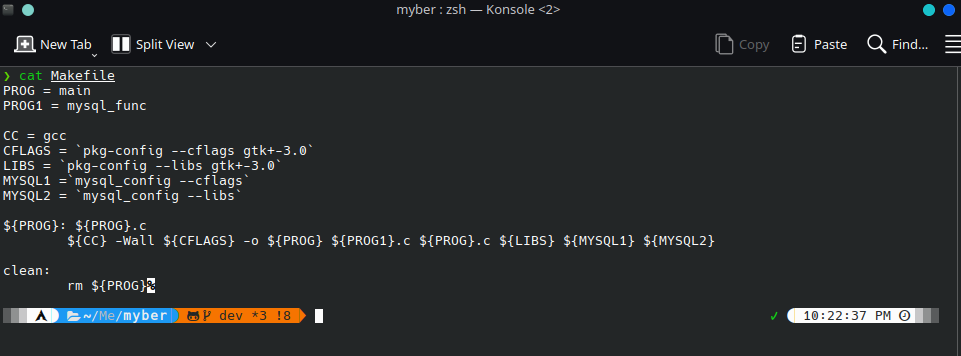
\includegraphics[width=1\textwidth]{./Makefile.png}
    \caption{Makefile}

\end{figure}
\FloatBarrier 

Selanjutnya untuk melakukan kompilasi, gunakan perintah berikut :

\begin{lstlisting}[language=bash]
make
\end{lstlisting}

\begin{figure}[!htbp]
    \centering
    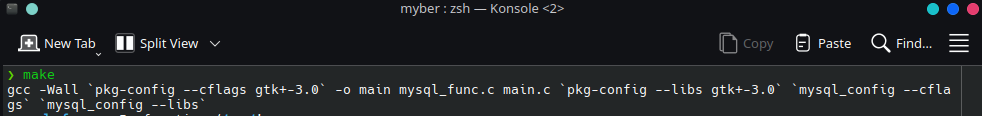
\includegraphics[width=1\textwidth]{./Make.png}
    \caption{Make}

\end{figure}
\FloatBarrier

Selanjutnya file binary program akan dihasilkan dari proses kompilasi, untuk menjalankan gunakan perintah :

\begin{lstlisting}[language=bash]
    ./main
\end{lstlisting}

\begin{figure}[!htbp]
    \centering
    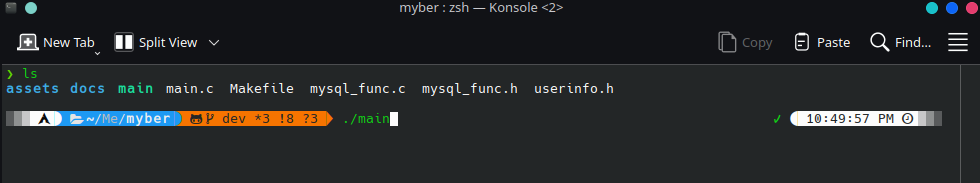
\includegraphics[width=1\textwidth]{./Main.png}
    \caption{File program hasil kompilasi}

\end{figure}
\FloatBarrier 

\subsection{Welcome Screen}
Berikut ini adalah tampilan ketika aplikasi pertama kali dibuka

\begin{figure}[!htbp]
    \centering
    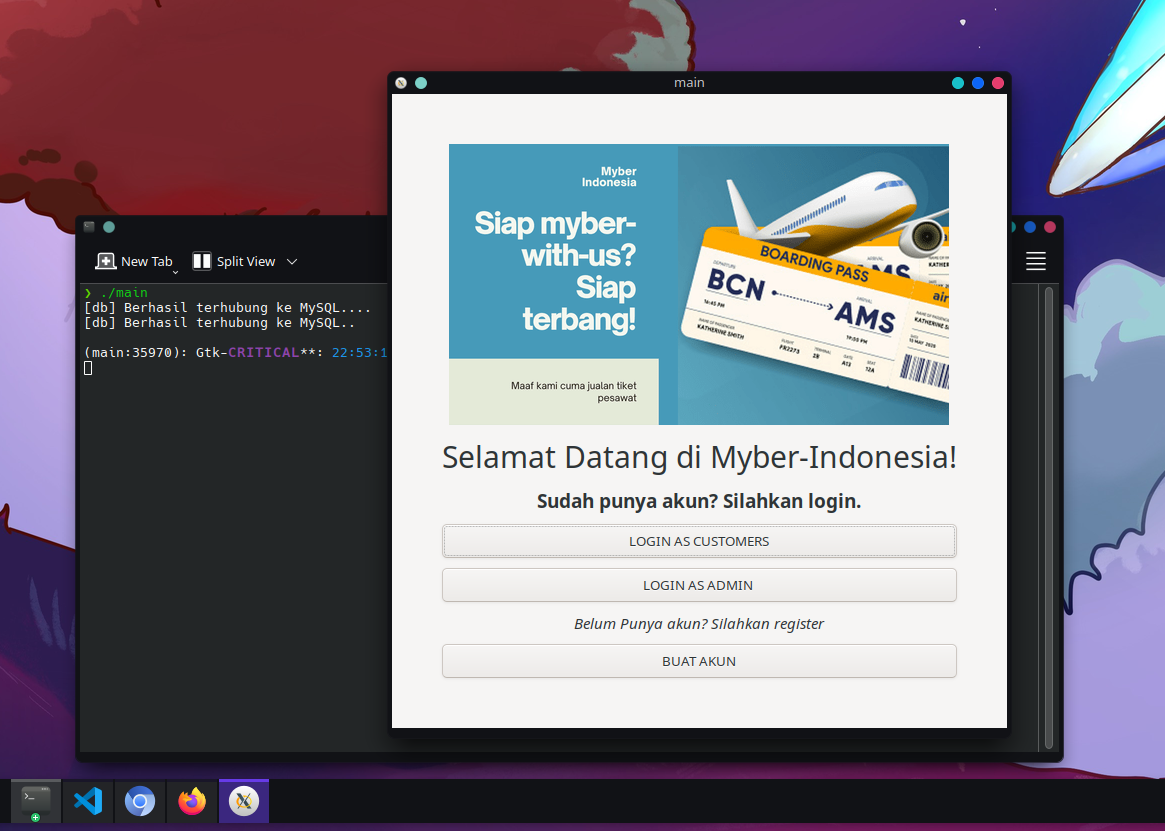
\includegraphics[width=1\textwidth]{./Welcome.png}
    \caption{File program hasil kompilasi}

\end{figure}
\FloatBarrier 

\subsection{Admin - Halaman Login}
Selanjutnya adalah halaman login admin, dengan tampilan sebagai berikut:
\begin{figure}[!htbp]
    \centering
    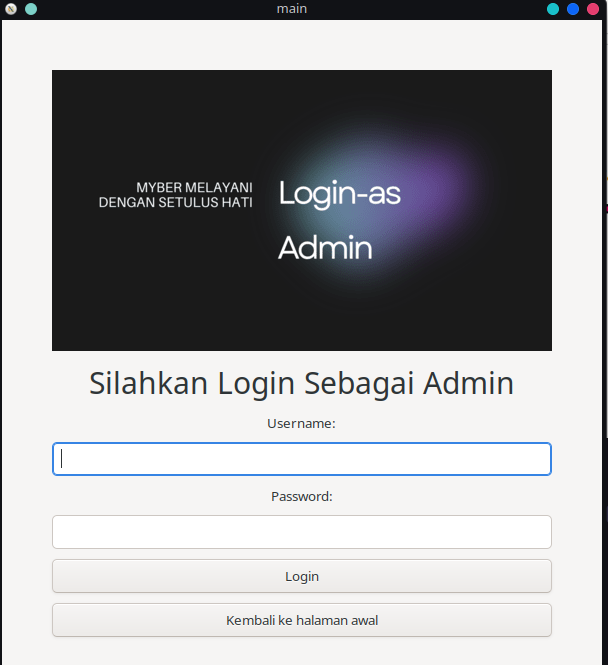
\includegraphics[width=0.43\textwidth]{./Login_admin.png}
    \caption{Halaman Login Admin}

\end{figure}
\FloatBarrier 

\subsection{Admin - Tampilan Awal}
Ini merupakan tampilan awal atau welcome screen Admin
\begin{figure}[!htbp]
    \centering
    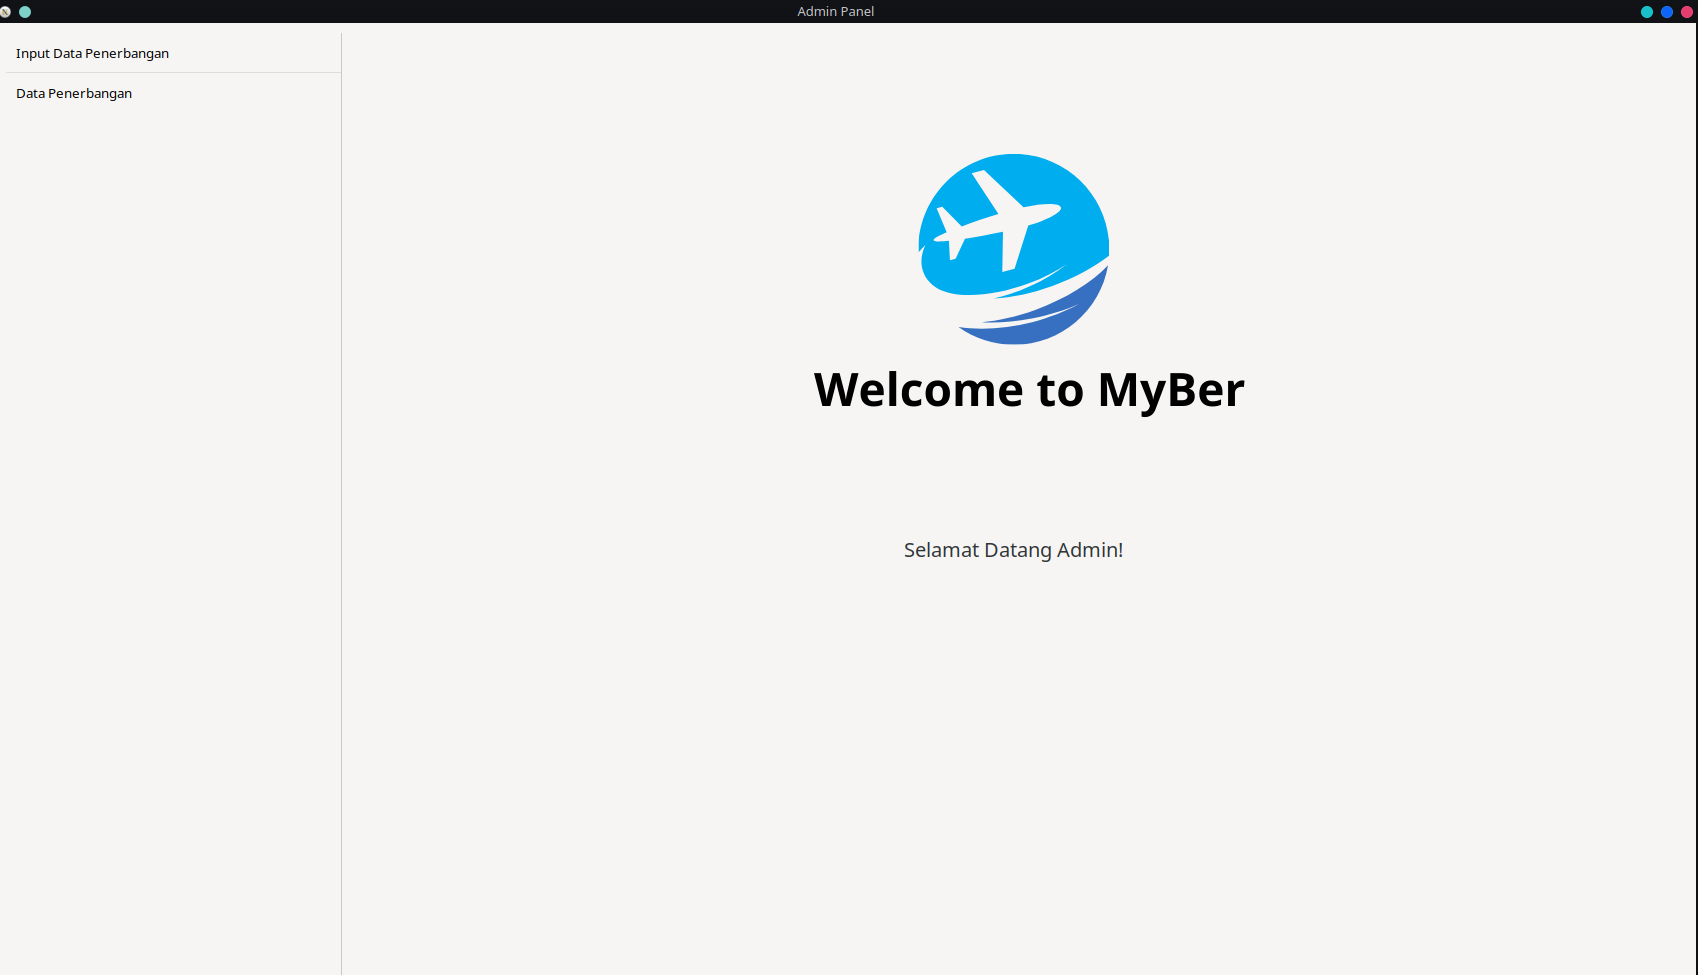
\includegraphics[width=0.9\textwidth]{./Home_Admin.png}
    \caption{Welcome Admin}

\end{figure}
\FloatBarrier 

\subsection{Admin - Input Data Pembelian}
Ini merupakan halaman untuk input data pembelian tiket oleh Admin
\begin{figure}[!htbp]
    \centering
    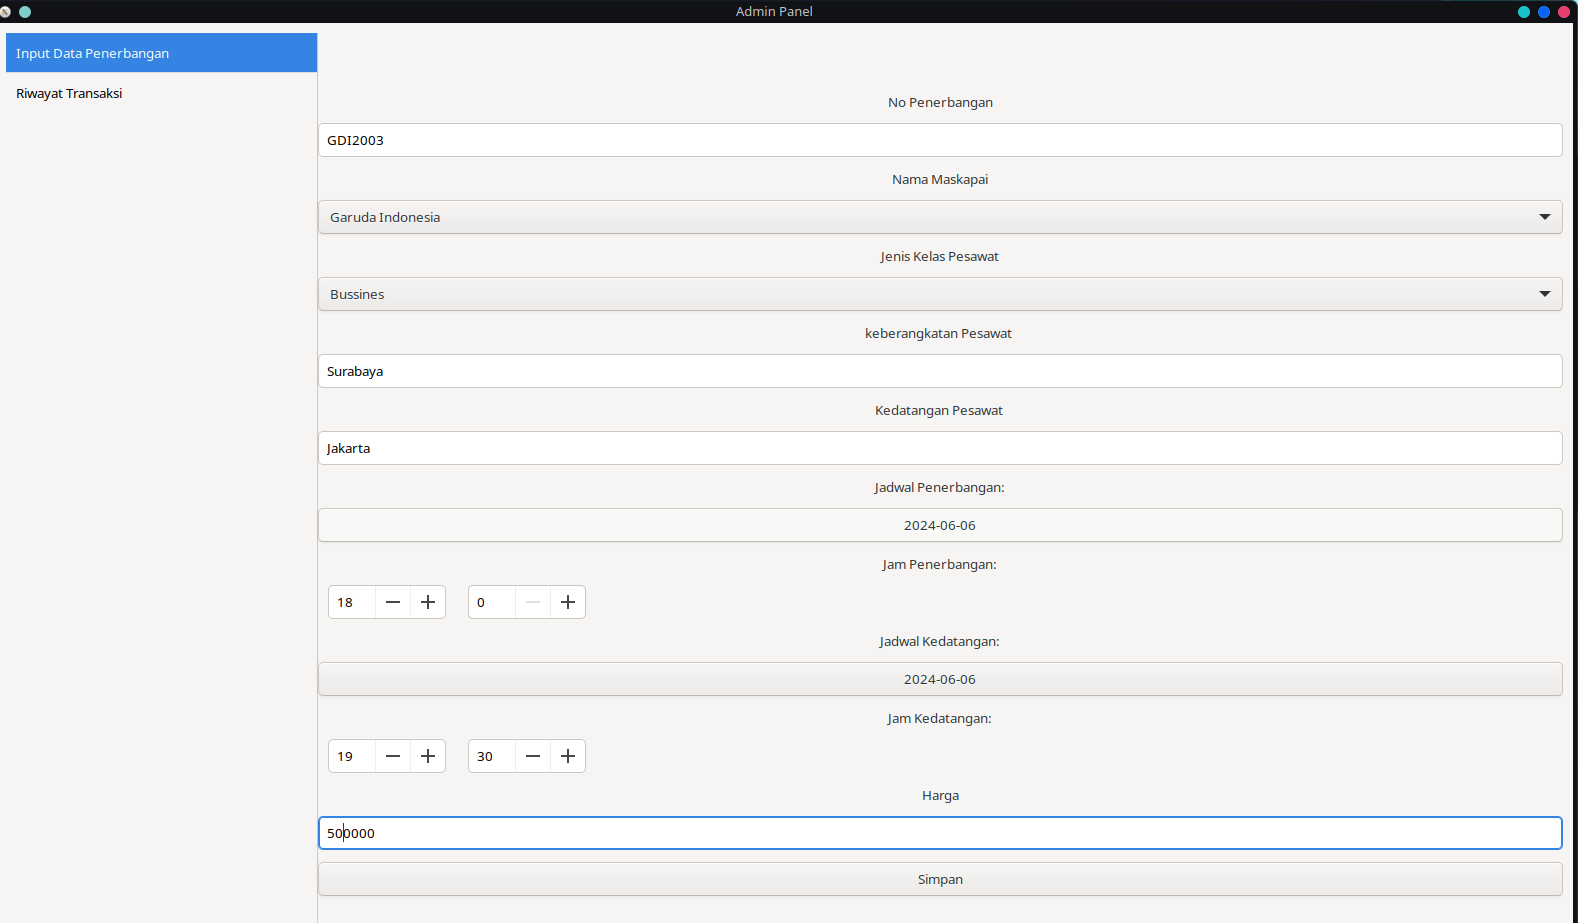
\includegraphics[width=0.9\textwidth]{./Input_data.png}
    \caption{Halaman Input Data Admin}

\end{figure}
\FloatBarrier 

\subsection{Admin - Data Penerbangan}
Ini merupakan halaman data penerbangan yang sebelumnya diinputkan oleh Admin
\begin{figure}[!htbp]
    \centering
    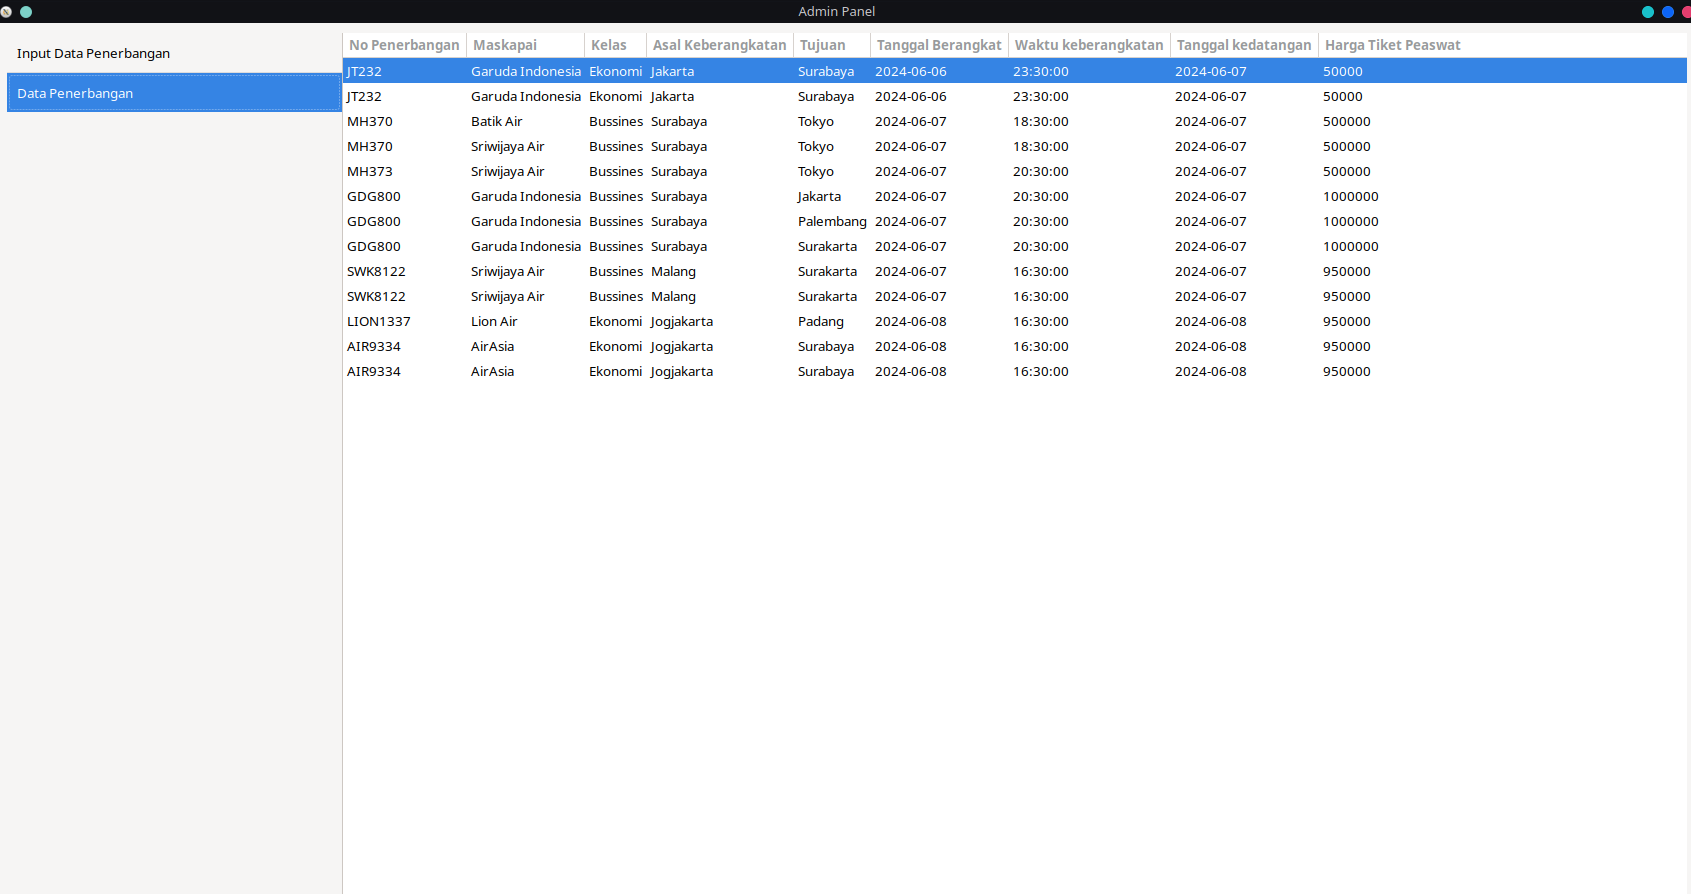
\includegraphics[width=0.9\textwidth]{./Data_penerbangan.png}
    \caption{Halaman Input Data Admin}

\end{figure}
\FloatBarrier 

\subsection{Customer - Halaman Register}
Berikut merupakan tampilan halaman register untuk pengguna/customer
\begin{figure}[!htbp]
    \centering
    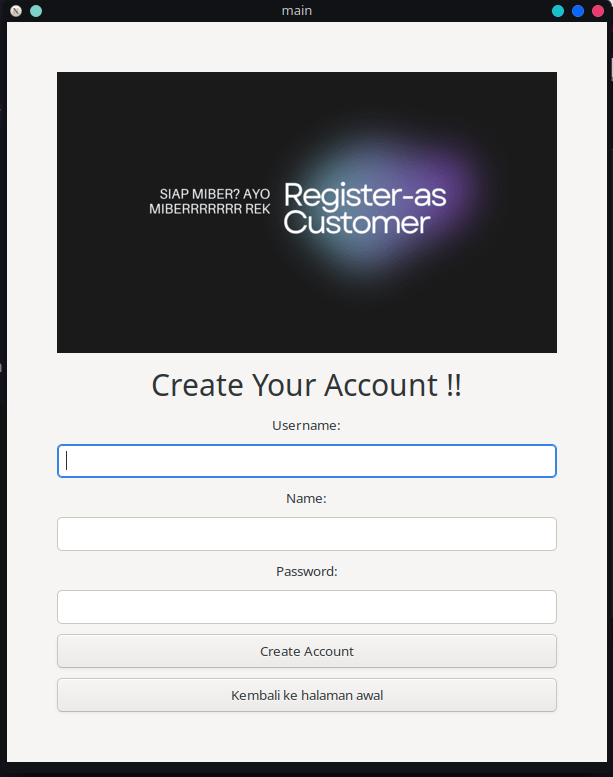
\includegraphics[width=0.45\textwidth]{./Register.png}
    \caption{Halaman Register Customer}

\end{figure}
\FloatBarrier 

\subsection{Customer - Halaman Login}
Ini merupakan tampilan halaman login untuk pengguna/customer
\begin{figure}[!htbp]
    \centering
    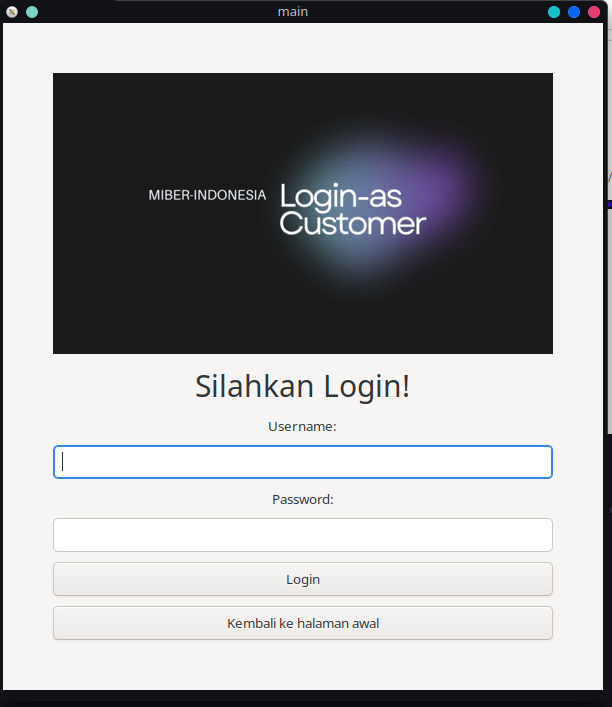
\includegraphics[width=0.45\textwidth]{./Login.png}
    \caption{Halaman Login Customer}

\end{figure}
\FloatBarrier 

\subsection{Customer - Tampilan Awal}
Berikut adalah tampilan ketika user selesai login
\begin{figure}[!htbp]
    \centering
    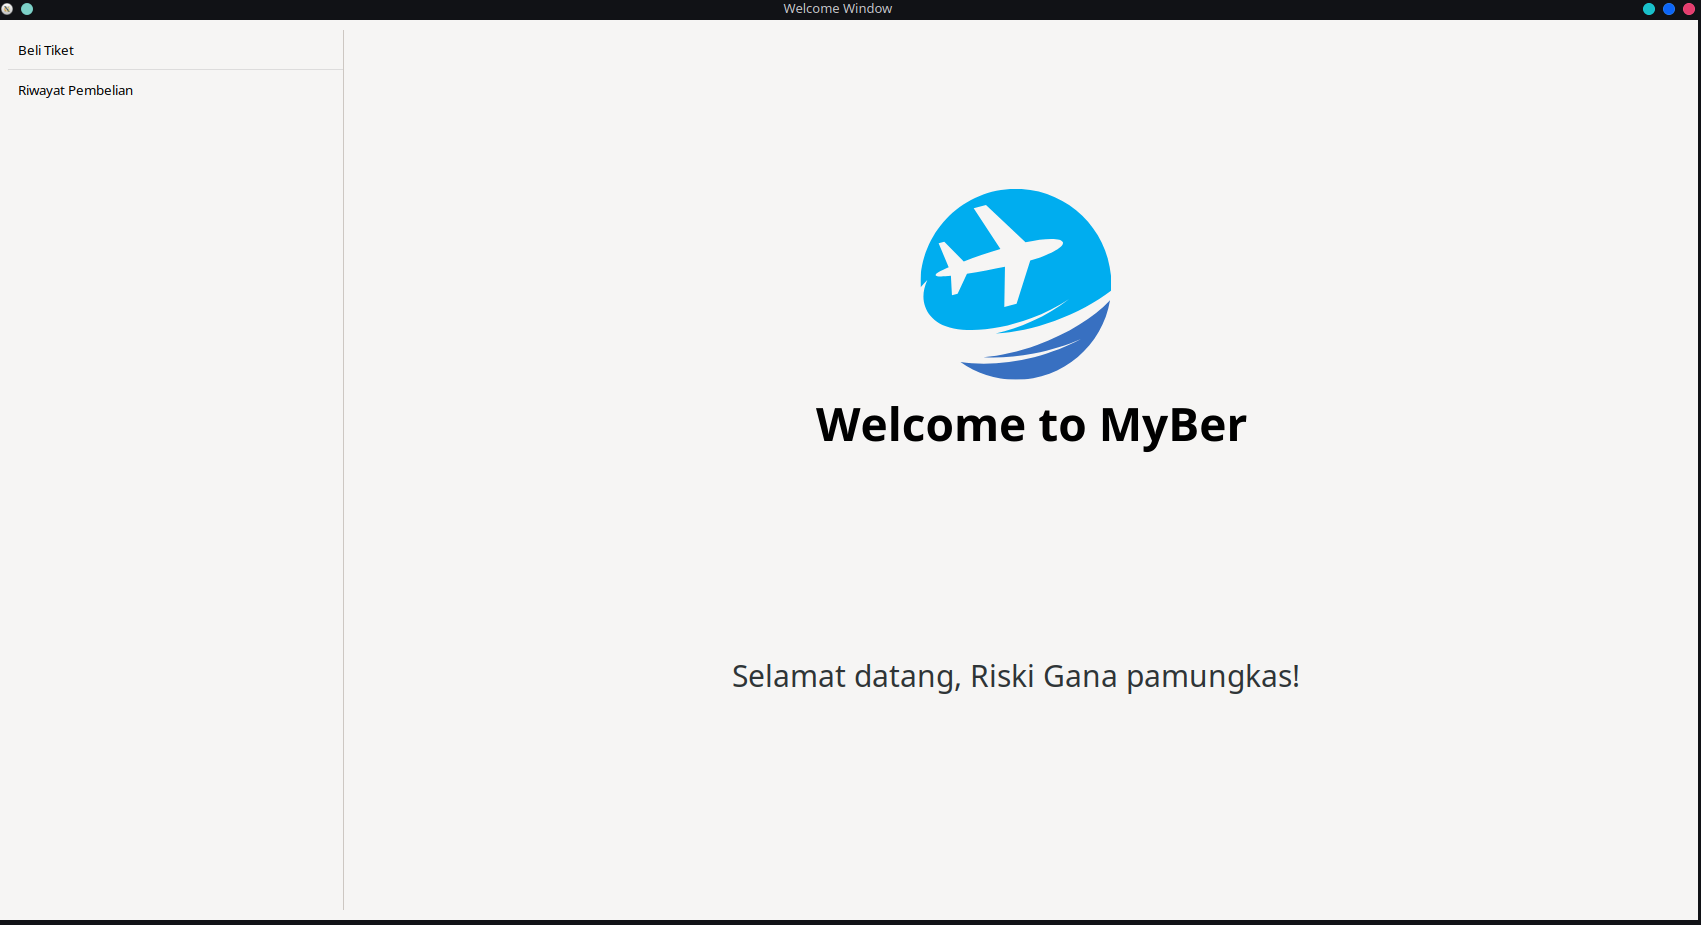
\includegraphics[width=0.8\textwidth]{./Home_User.png}
    \caption{Halaman Utama User}

\end{figure}
\FloatBarrier 

\subsection{Customer - Halaman Pembelian Tiket}
Ini merupakan tampilan halaman pembelian tiket
\begin{figure}[!htbp]
    \centering
    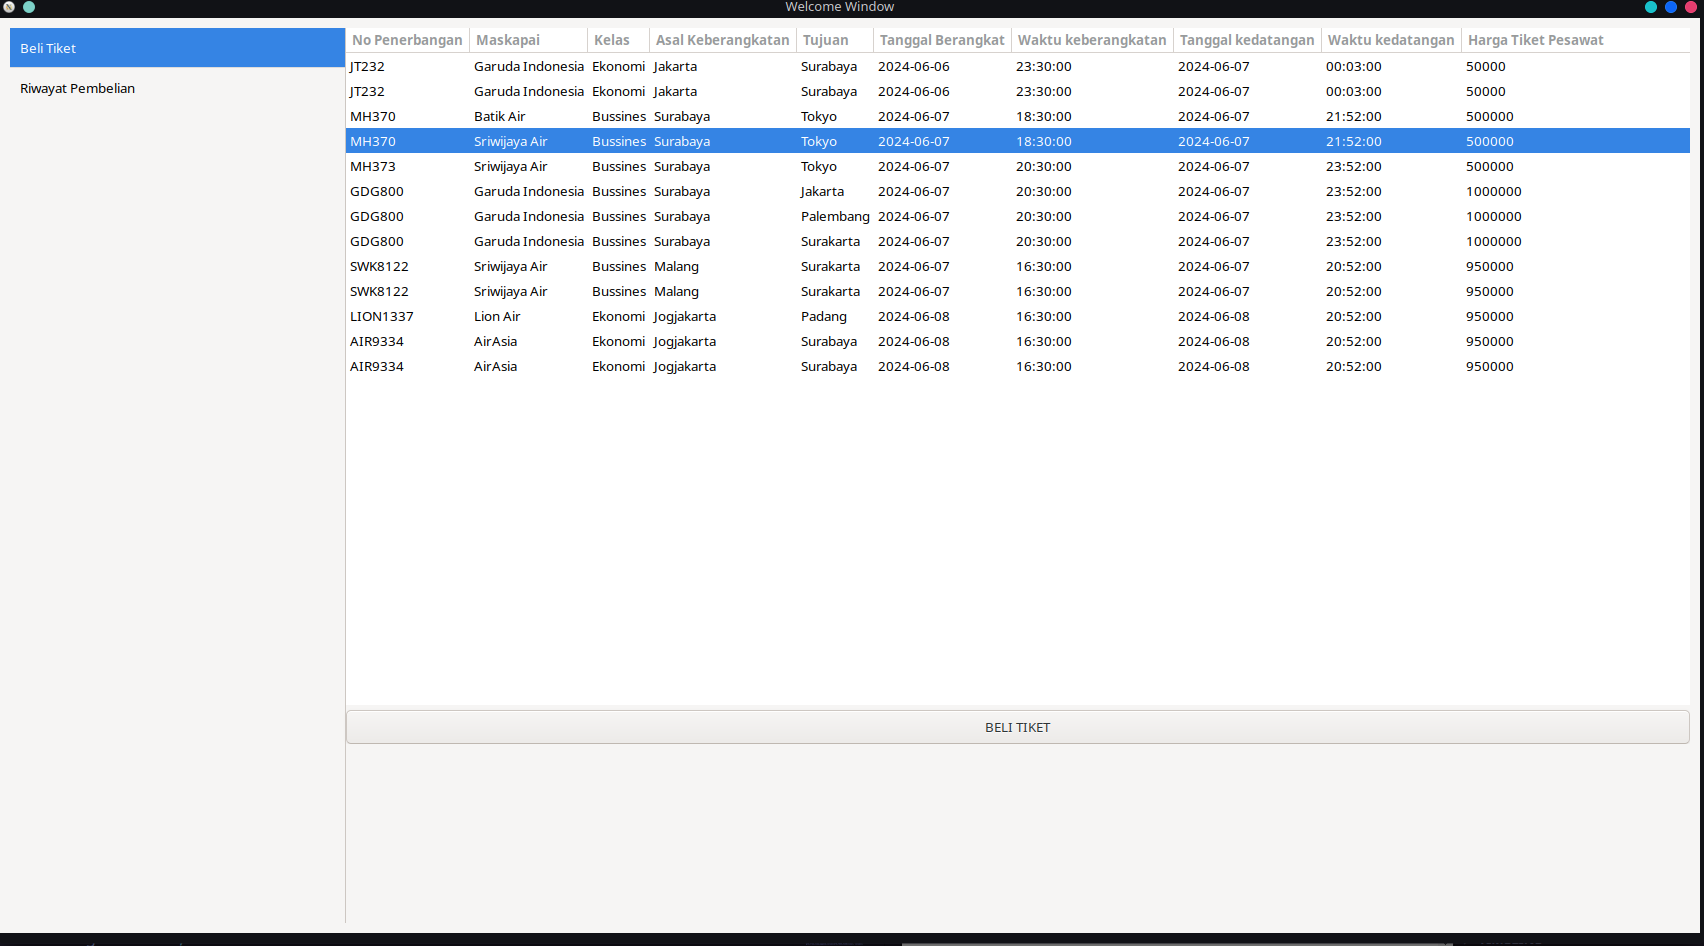
\includegraphics[width=0.8\textwidth]{./Beli_tiket.png}
    \caption{Halaman Pembelian Tiket}

\end{figure}
\FloatBarrier 

\subsection{Customer - Riwayat Pembeliam Tiket}
Ini merupakan tampilan dari riwayat pembelian tiket oleh Customer
\begin{figure}[!htbp]
    \centering
    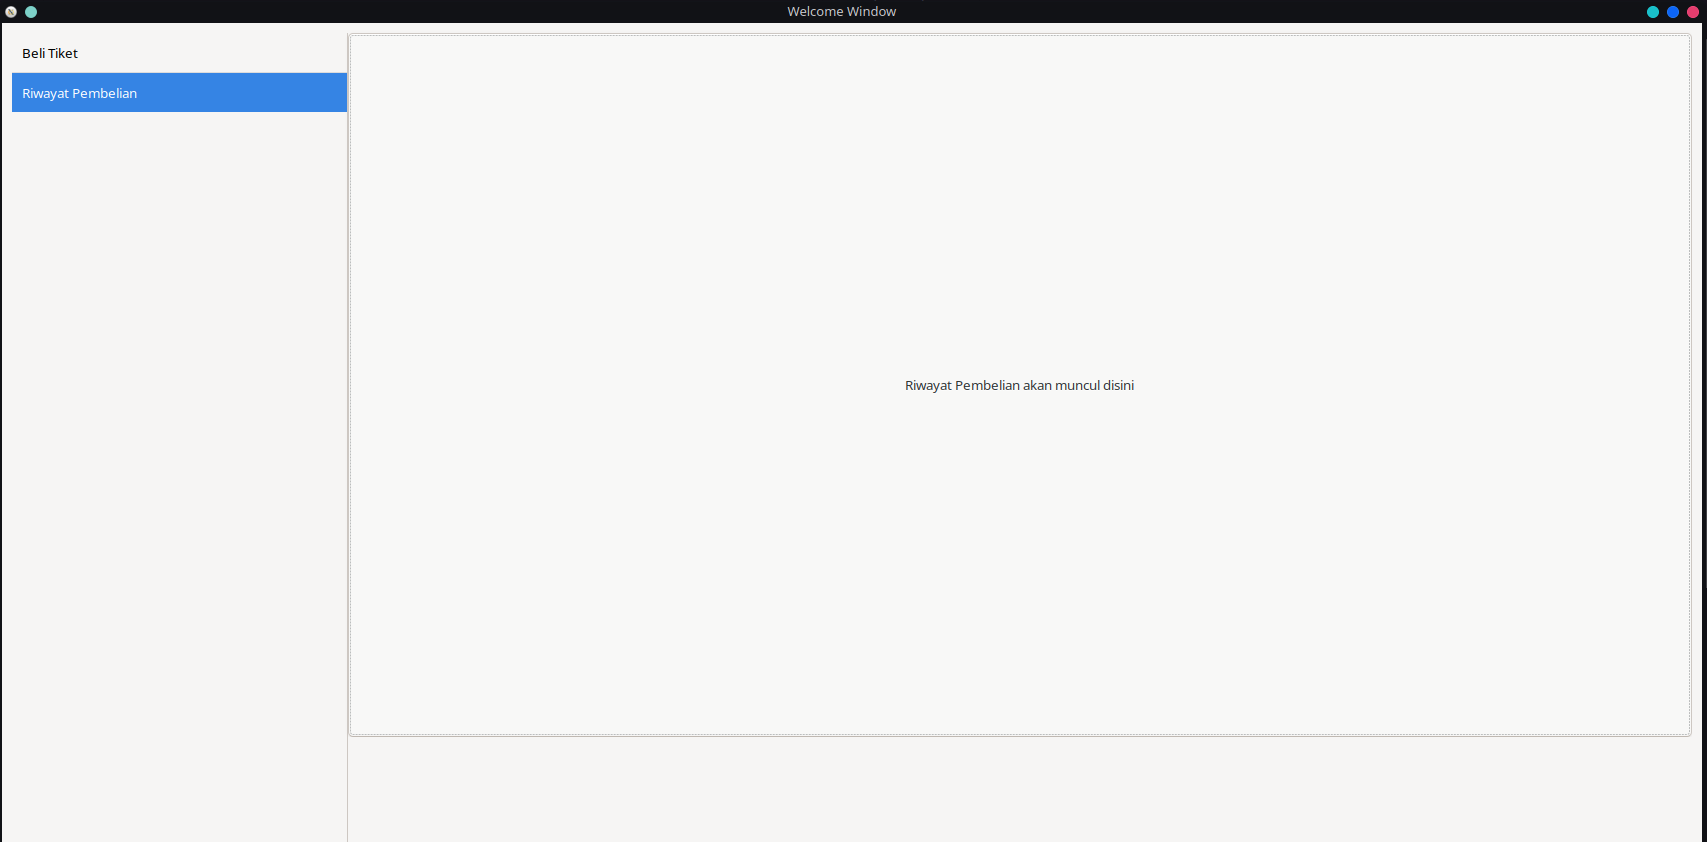
\includegraphics[width=0.8\textwidth]{./Riwayat-User.png}
    \caption{Halaman Pembelian Tiket}

\end{figure}
\FloatBarrier 

\section{Kode Program}
Kode program dari aplikasi kami lampirkan dalam folder myber beserta file myber-dev.zip, serta pada repository github berikut :
\begin{itemize}
    \item \url{https://github.com/indonumberone/myber}
\end{itemize}

\section{Analisa}

\subsection{Alur Program}
Setelah melakukan kompilasi dan compiler menghasilkan sebuah file main. Selanjutnya adalah melakukan eksekusi file binary tersebut. Keseluruhan alur dari aplikasi ini adalah sebagai berikut.

\subsubsection{Welcome Screen}
Welcome screen merupakan tampilan awal ketika menjalankan aplikasi ini.

\begin{figure}[!htbp]
    \centering
    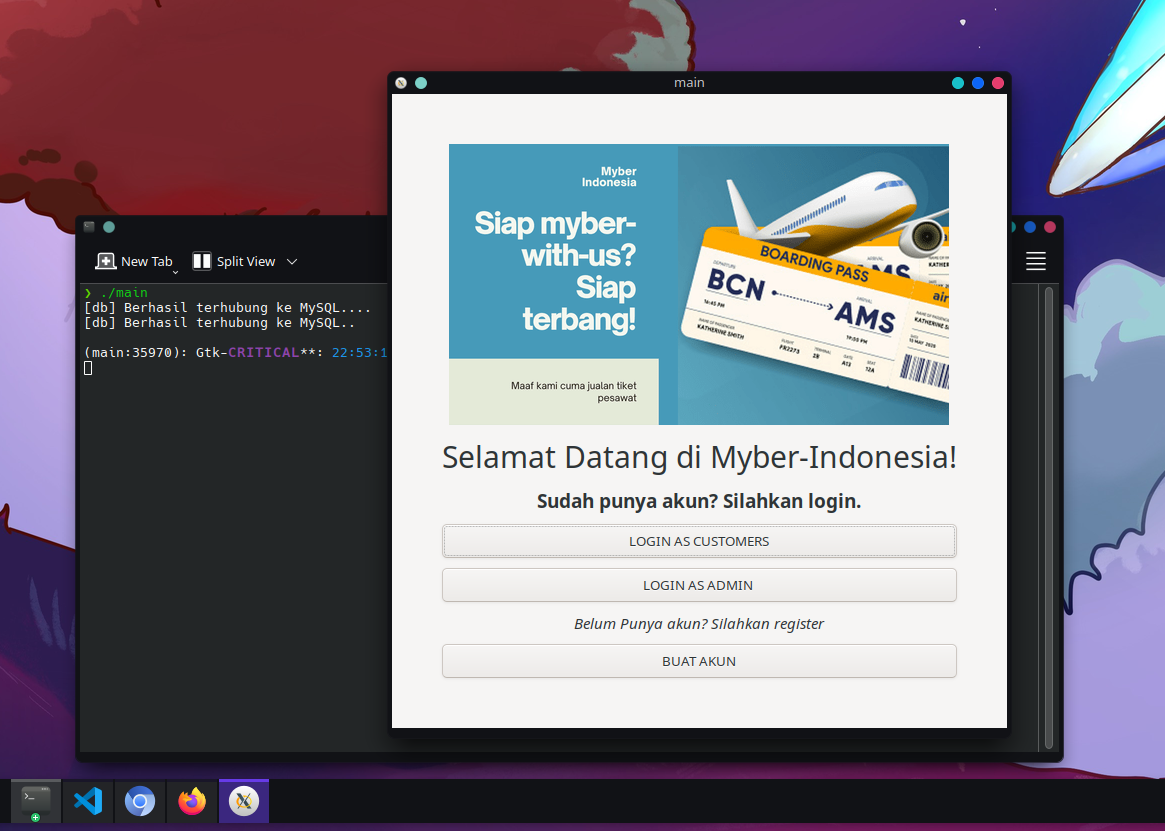
\includegraphics[width=0.5\textwidth]{./Welcome.png}
    \caption{Welcome Screen}

\end{figure}
\FloatBarrier 

Pengguna dalam hal ini ada dua tipe pengguna yaitu Admin dan Customer. 
Dari sisi Customer, terdapat dua buah fungsi pada bagian ini yaitu untuk Register dan Login.
Sedangkan dari sisi Admin hanya bisa melakukan login, karena kredensial Admin sudah dibuat secara terpisah pada database.

Kode dari halaman ini terdapat dalam fungsi utama yaitu main pada file main.c 
\begin{figure}[!htbp]
    \centering
    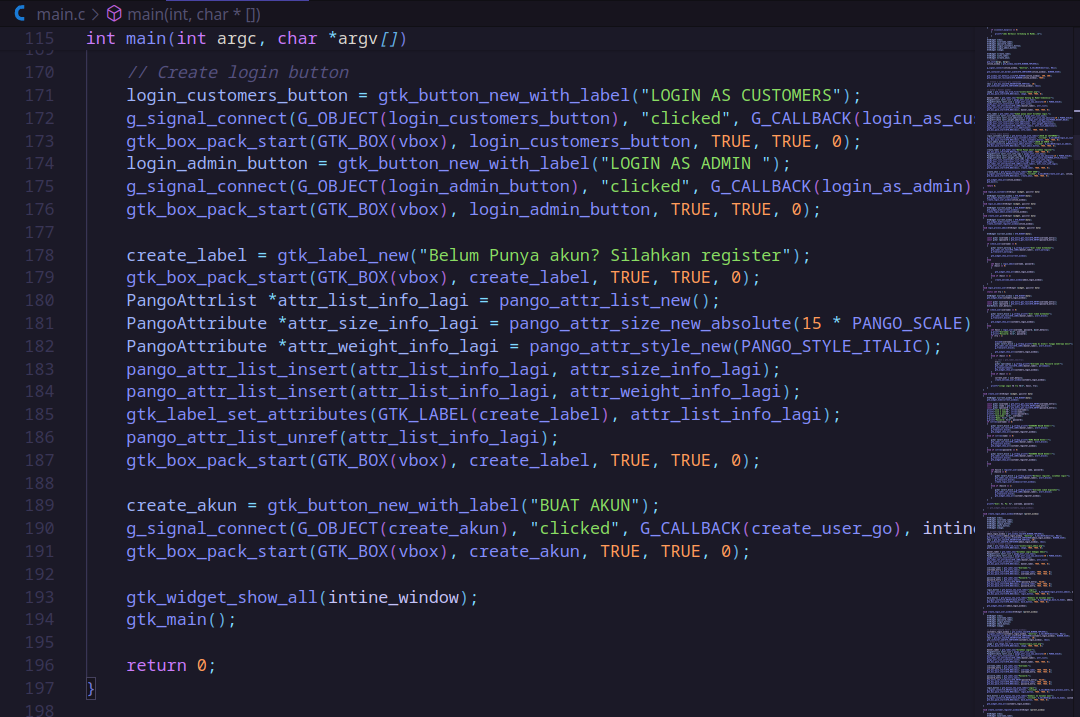
\includegraphics[width=0.5\textwidth]{./docs_main.png}
    \caption{Sebagian Kode Program untuk Welcome Screen}

\end{figure}
\FloatBarrier 

Kode tersebut memanggil beberapa entitas dari GTK seperti membuat window beserta memanggil GtkWidget yang merupakan base class dari widget yang ada pada GTK.
Dari GtkWidget kemudian bisa dibuat beberapa elemen lain yang nantinya akan membentuk user interface dari aplikasi ini.

Contohnya adalah dalam pembuatan teks atau tulisan, teks dalam GTK disebut sebagai label. Untuk membuat label pertama yang dilakukan adalah memanggil GtkLabel lalu menggunakan Constructor new dari GtkLabel untuk membuat sebuah label baru.

\begin{figure}[!htbp]
    \centering
    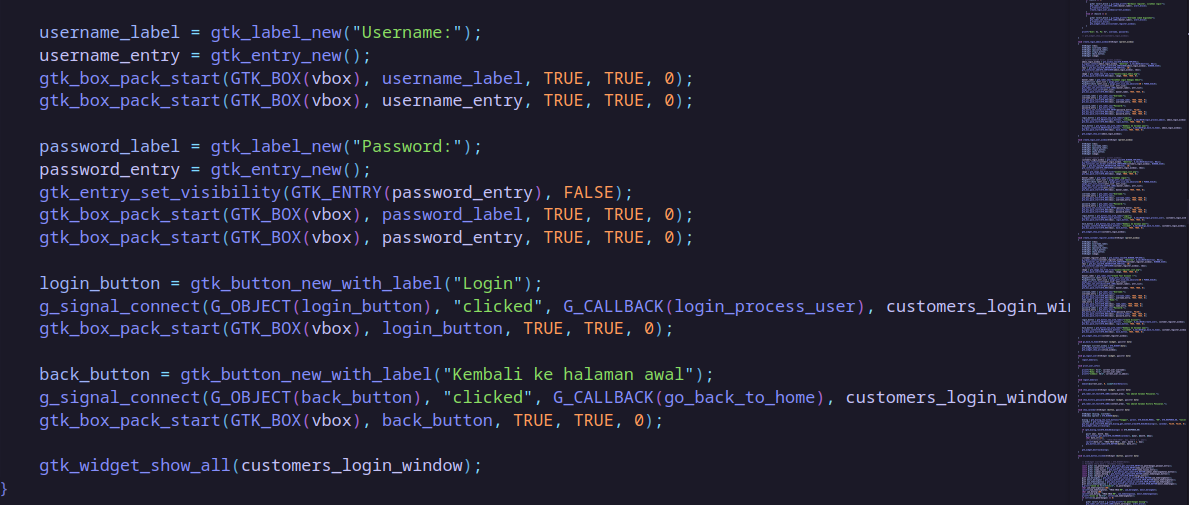
\includegraphics[width=0.5\textwidth]{./docs_label.png}
    \caption{GtkLabel}

\end{figure}
\FloatBarrier 

Sebagai contoh, diatas merupakan kode program dari fungsi \texttt{\detokenize{create_login_user_window()}}
Teks-teks seperti Username, Password, Login dan Kembali ke halaman awal dibuat dengan menggunakan GtkLabel. Dimana dalam membuat Constructor adalah dengan memanggil fungsi
\texttt{\detokenize{gtk_label_new("isi_teks);}}. Setelah itu adalah menampilkannya ke dalam window dengan memanggil fungsi \texttt{\detokenize{gtk_widget_show_all(window_saat_ini)}}
Dokumentasi dari GtkLabel yang lebih lengkap terdapat pada halaman \url{https://docs.gtk.org/gtk3/ctor.Widget.new.html}
\subsection{Halaman Register}
Pada Halaman Register digunakan user untuk membuat akun aplikasi MyBer.
\begin{figure}[!h]
    \centering
    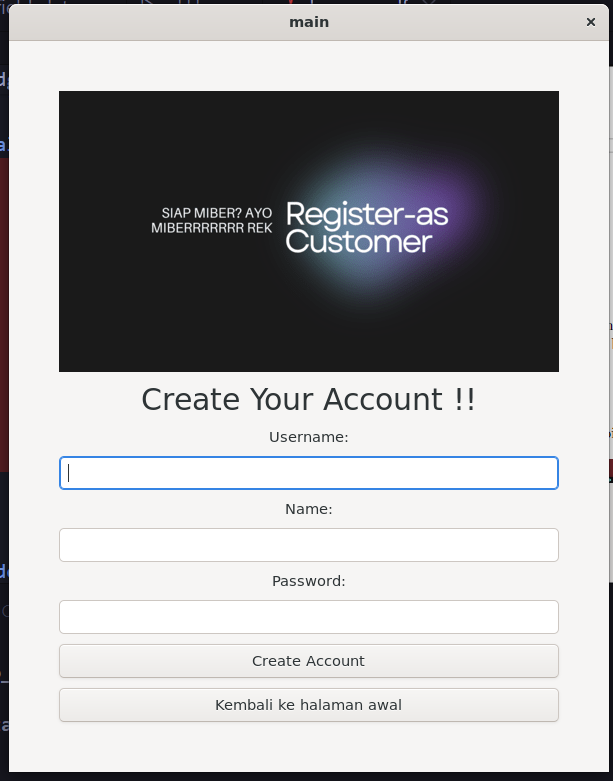
\includegraphics[width=0.45\textwidth]{./img/create_user_screen.png}
    \caption{Halaman Register}
\end{figure}
\FloatBarrier
Pada halaman ini jika user ingin membuat sebuah akun maka wajib mengisi semua text input yang disediakan, jika user belum menginputkan semua text input yang digunakan maka akan alert atau warning yang muncul, seperti berikut ini:
\begin{figure}[!h]
    \centering
    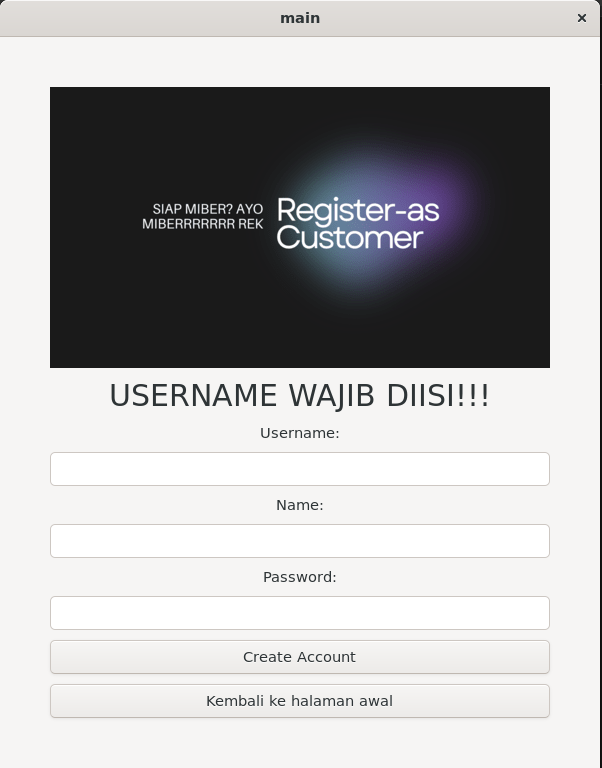
\includegraphics[width=0.5\textwidth]{./img/username_kosong.png}
    \caption{Username kosong}
\end{figure}
\FloatBarrier
Pada gambar diatas terjadi ketika user tidak menginputkan username
\begin{figure}[!htbp]
    \centering
    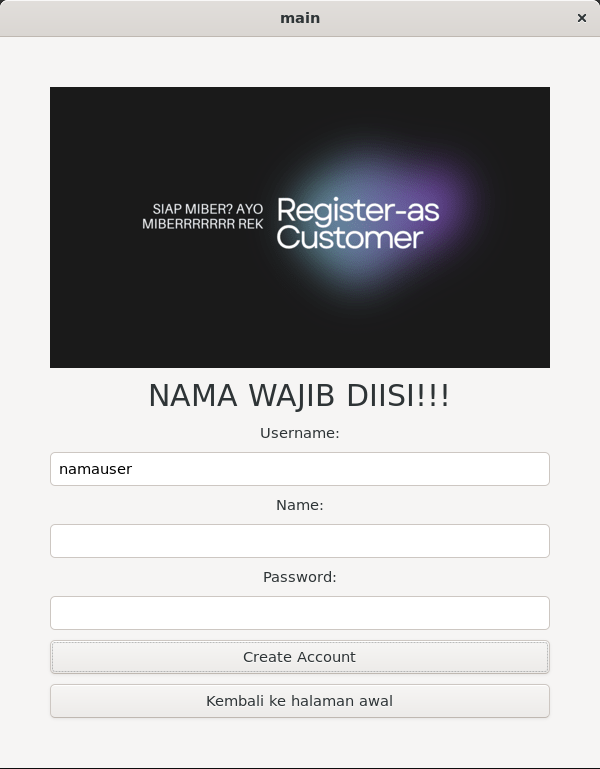
\includegraphics[width=0.45\textwidth]{./img/nama_kosong.png}
    \caption{nama kosong}
\end{figure}
\FloatBarrier
Pada gambar diatas terjadi ketika user tidak menginputkan nama 
\begin{figure}[htbp]
    \centering
    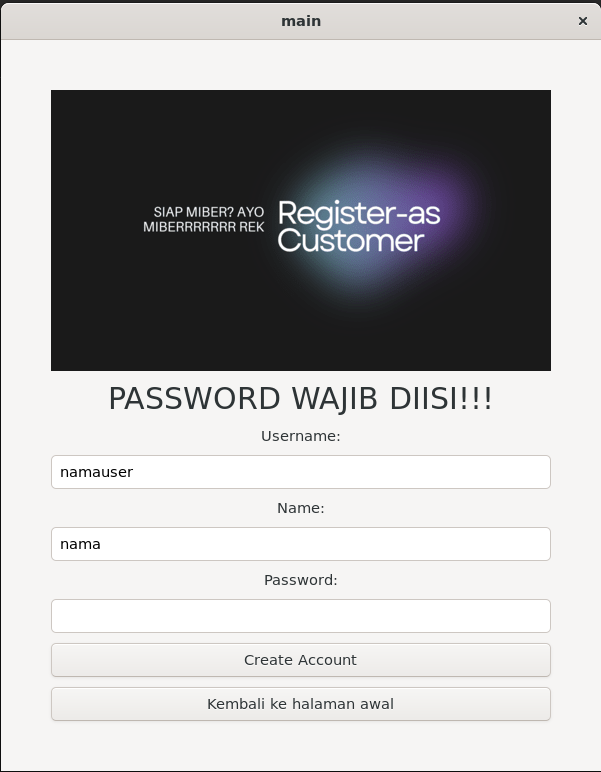
\includegraphics[width=0.4\textwidth]{./img/password_kosong.png}
    \caption{password kosong}
\end{figure}
\FloatBarrier
Pada gambar diatas terjadi ketika user tidak menginputkan password
\begin{figure}[!htbp]
    \centering
    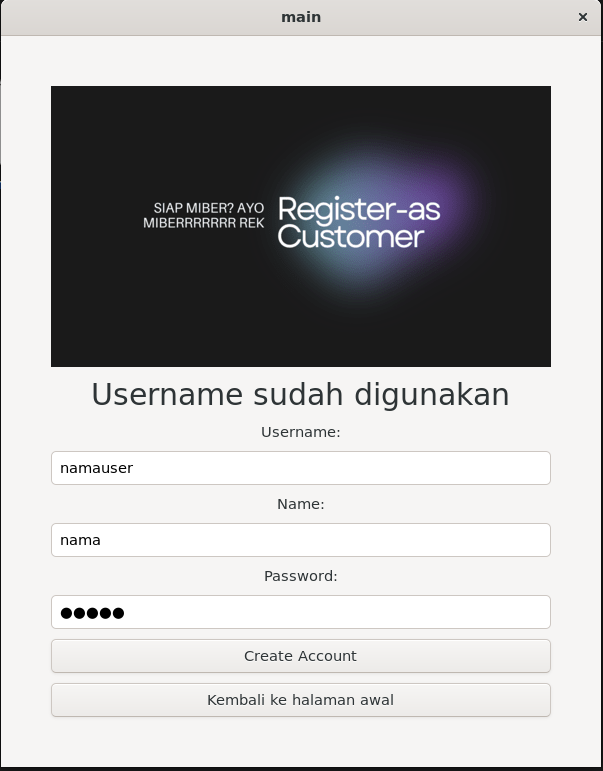
\includegraphics[width=0.4\textwidth]{./img/username_dipakai.png}
    \caption{username telah dipakai}
\end{figure}
\FloatBarrier
Pada gambar diatas terjadi ketika username yang diinputkan oleh user telah dipakai oleh userlain.
\FloatBarrier
Berikut ini adalah tampilan kode dari halaman register
\begin{figure}[!htbp]
    \centering
    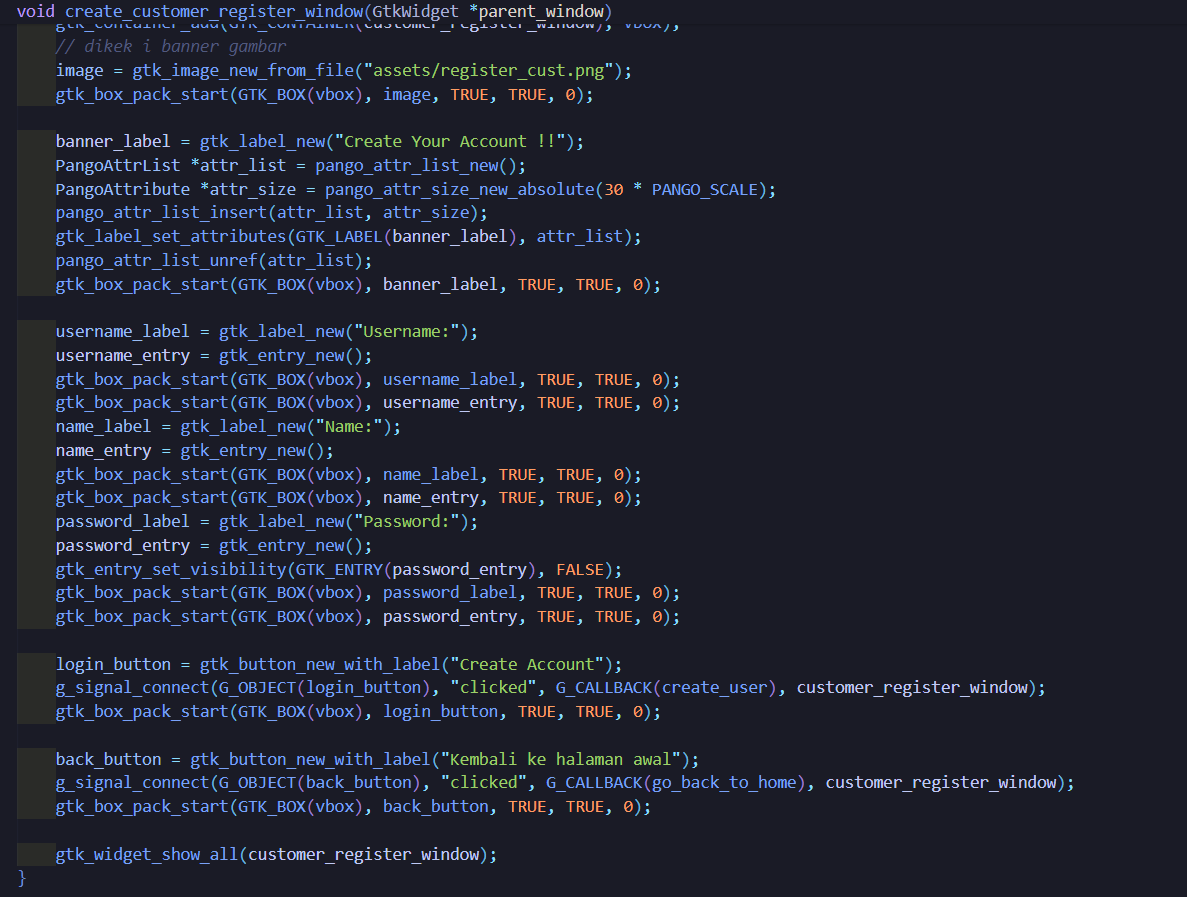
\includegraphics[width=0.5\textwidth]{./img/kode_halaman_register_gtk.png}
    \caption{Kode halaman register dari gtk}
\end{figure}
\FloatBarrier
Dari kode diatas dibuat sebuah window bernama \texttt{\detokenize{customer_register_window()}} yang digunakan
sebagai window pada halaman register. kemudian dibuat sebuah box dengan nama vbox dengan orientasi vertikal yang dimasukan ke dalam container window,
dibuat box dengan orientasi vertikal ini bertujuan agar setiap ada widget baru yang nantinya akan ditambahkan ke dalam
vbox ini akan tertata secara vertikal menurun.

kemudian variabel yang berisi fungsi gtk entry new digunakan untuk mengambil teks yang diinputkan oleh user,kemudian jika user menekan button create akun maka
maka fungsi callback dari button akan mengarahkan ke fungsi create user
\begin{figure}[!htbp]
    \centering
    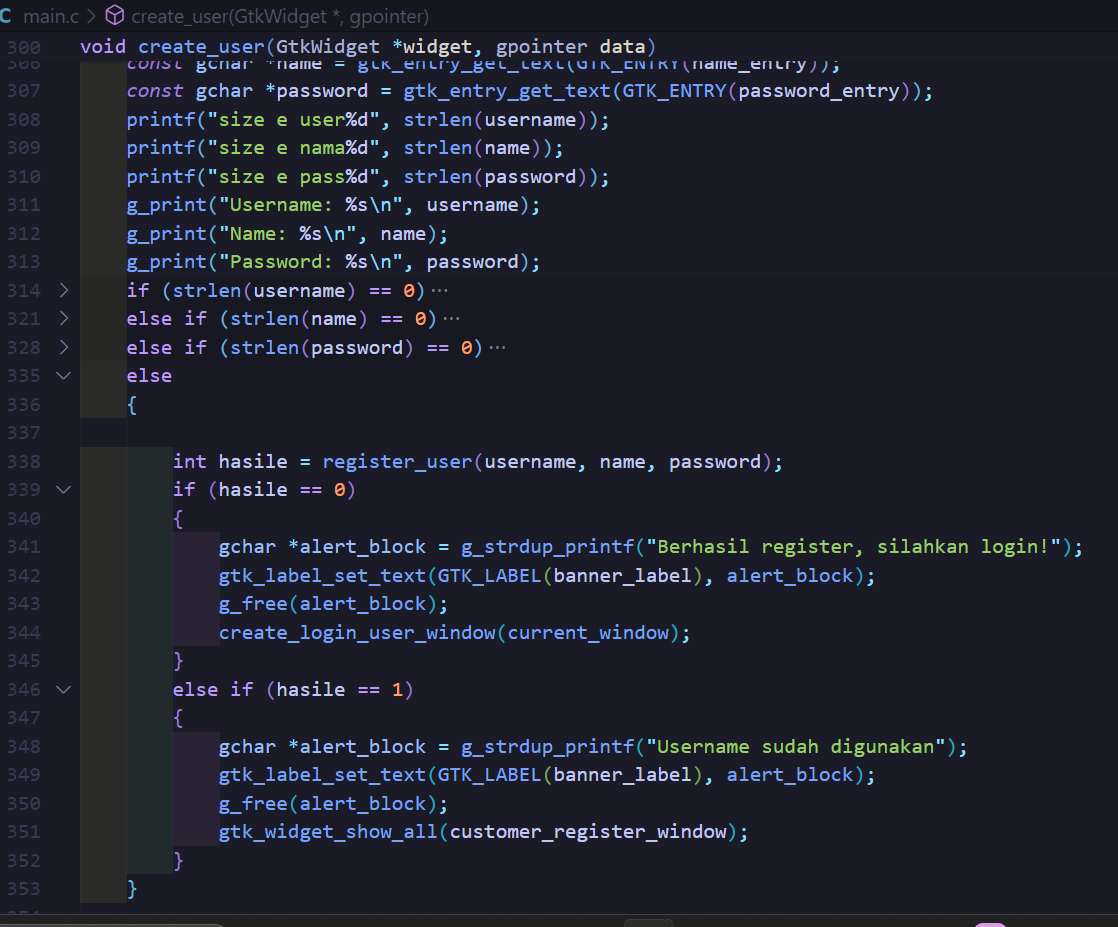
\includegraphics[width=0.5\textwidth]{./img/kode_fungsi_createuser.png}
    \caption{Kode dari fungsi create user}
\end{figure}
\FloatBarrier
Dari kode diatas username yang telah diinputkan akan di ambil dan disimpan dalam sebuah variabel seperti username,nama.password, dari variabel tersebut kemudian di cek apakah
panjang dari variabel(variabel username,nama,password) sama dengan 0 jika sama dengan 0 maka akan mengganti nilai label yang awalanya berisi
Create Your Account!!,pengecekan ini bertujuan agar user yang ingin membuat sebuah akun wajib mengisi text input yang disediakan, jika user telah mengisi
semua text input yang digunakan maka variabel tadi akan dijadikan argumen untuk fungsi register user
\begin{figure}[!htbp]
    \centering
    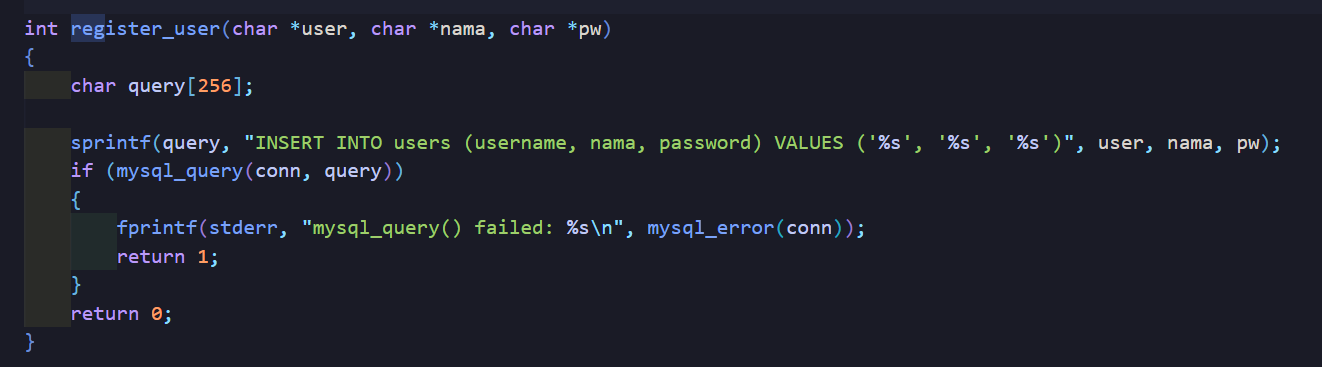
\includegraphics[width=0.5\textwidth]{./img/register_user.png}
    \caption{Kode untuk menginputkan data kedalam mysql}
\end{figure}
\FloatBarrier
Dari kode diatas digunakan untuk menginputkan kedalam database mysql dengan menggunakan insert into, jika username ada yang sama akan mengembalikan 1 jika username tidak ada yang sama maka akan mengembalikan 
nilai 0 dari nilai diatas di kembalikan ke fungsi create user dan kemudian di handling jika pengembalian fungsi regster user itu 1 maka akan username tersebut telah dipakai , jika 0 maka user berhasil mendaftar dan data berhasil 
disimpan dalam database mysql,dan akan diredirect ke halaman login.

\subsection{Halaman Login User}
Halaman Login User adalah halaman yang digunakan untuk user masuk kedalam akunya dan menuju ke dashboard tampiilan user
\begin{figure}[!htbp]
    \centering
    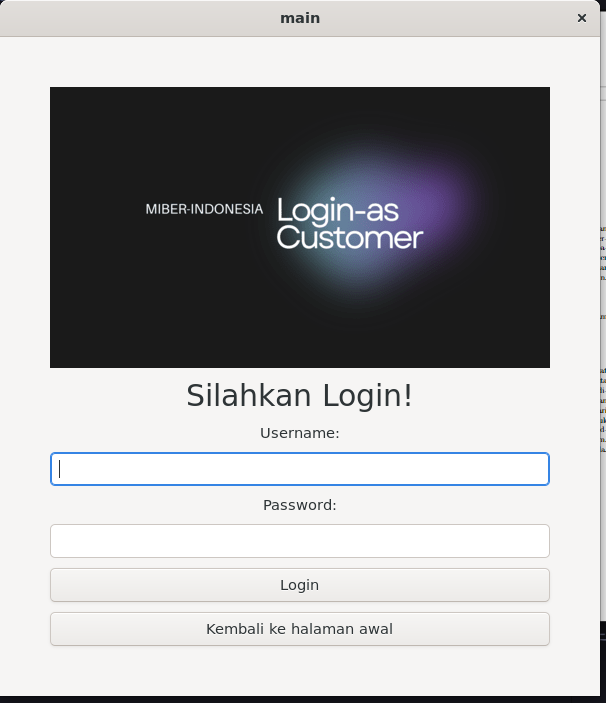
\includegraphics[width=0.5\textwidth]{./img/login_user.png}
    \caption{Tampilan Awal dari Login User}
\end{figure}
\FloatBarrier
Tampilan diatas adalah tampilan Login User, dari tampilan itu user disuruh untuk mengisi username dan password untuk masuk ke tampilan selanjutnya. Untuk melihat
logic pada tampilan ini bekerja kita bisa melihat di dalam fungsi beikut ini.
\begin{figure}[!htbp]
    \centering
    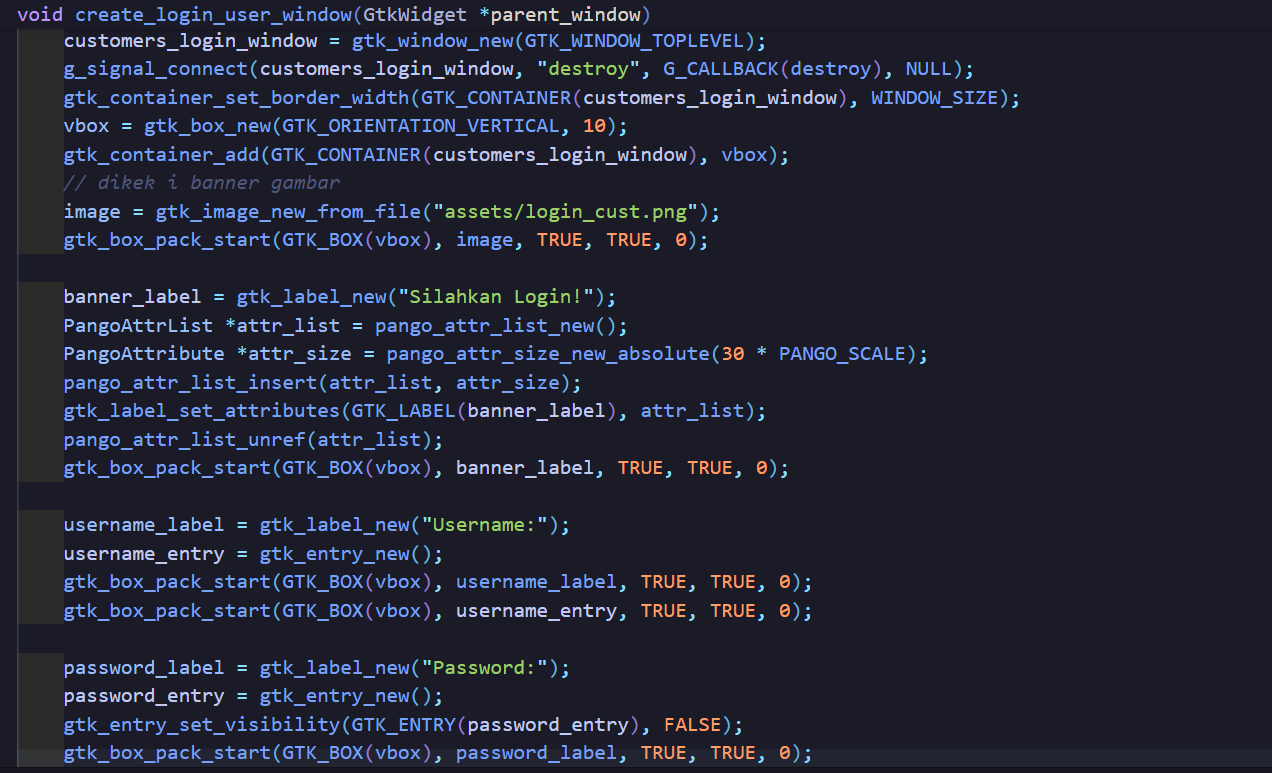
\includegraphics[width=0.5\textwidth]{./img/kode_login_user.png}
    \caption{Kode fungsi login user pada gtk}
\end{figure}
\FloatBarrier
Dari kode diatas \texttt{\detokenize{gtk_label_new()}} digunakan untuk memberikan tampilan teks ke gtk window yang telah dibuat
kemudian \texttt{\detokenize{gtk_entry_new()}} digunakan untuk menangkap text input yang diinputkan oleh user. kemudian \texttt{\detokenize{gtk_buuton_new_with_label()}}
digunakan untuk membuat sebuah button dengan text ditengah tengah button. ketika button itu di klik maka fungsi callback dari gtk akan memanggil fungsi \texttt{\detokenize{login_process_user()}} 
\begin{figure}[!htbp]
    \centering
    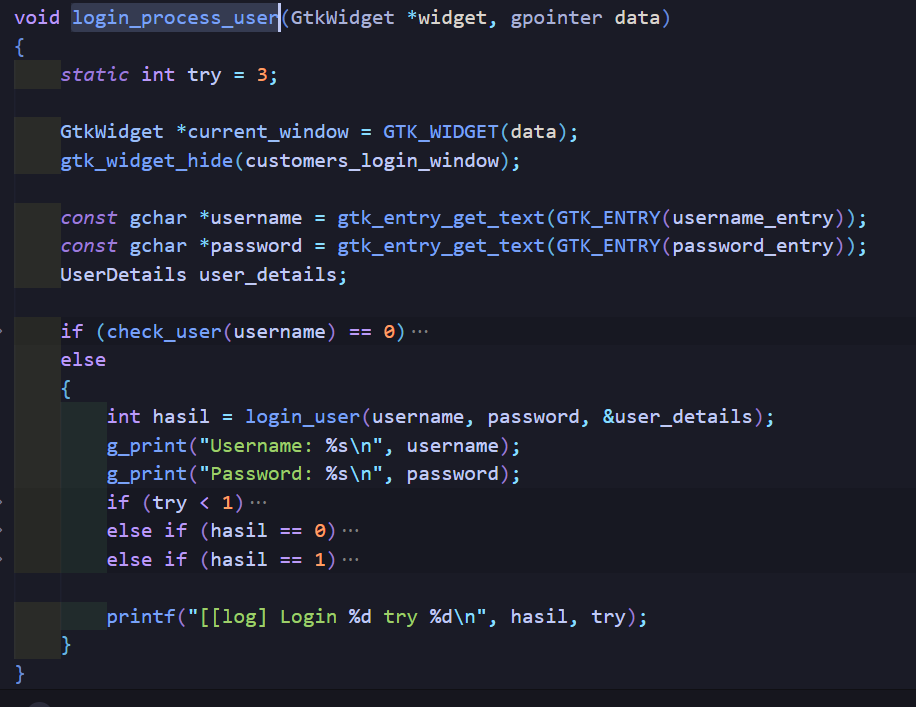
\includegraphics[width=0.5\textwidth]{./img/login_process_user.png}
    \caption{Kode dari login process user}
\end{figure}
\FloatBarrier
Dari kode diatas terdapat sebuah variabel statis dengan tipe data integer yang bernilai 3, kemudian terdapat variabel yang digunakan untuk mendapatkan text input username dan password
kemudian dari variabel variabel tersebut dijadikan argumen pada fungsi \texttt{\detokenize{check_user()}}

\begin{figure}[!htbp]
    \centering
    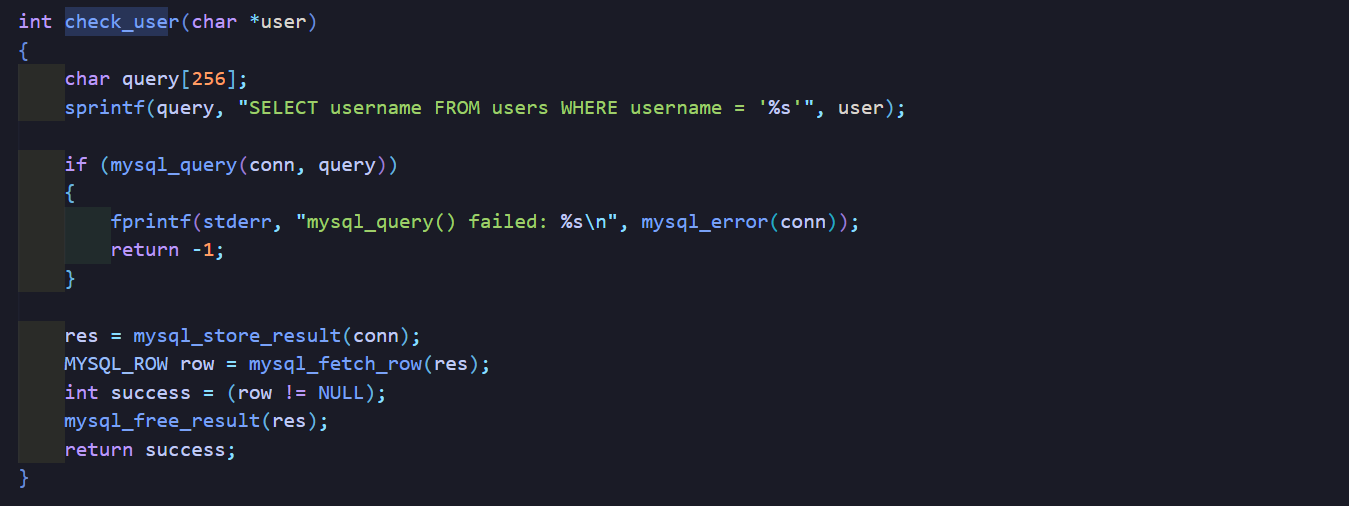
\includegraphics[width=0.5\textwidth]{./img/check_user_mysql.png}
    \caption{fungsi \texttt{\detokenize{check_user()}}}
\end{figure}
\FloatBarrier
fungsi \texttt{\detokenize{check_user()}} ini digunakan untuk mengecek pada databases apakah ada username sudah ada pada database belum.
jika ada maka lanjut keproses dibahwanya terdapat sebuah fungsi \texttt{\detokenize{login_user()}} 
\begin{figure}[!htbp]
    \centering
    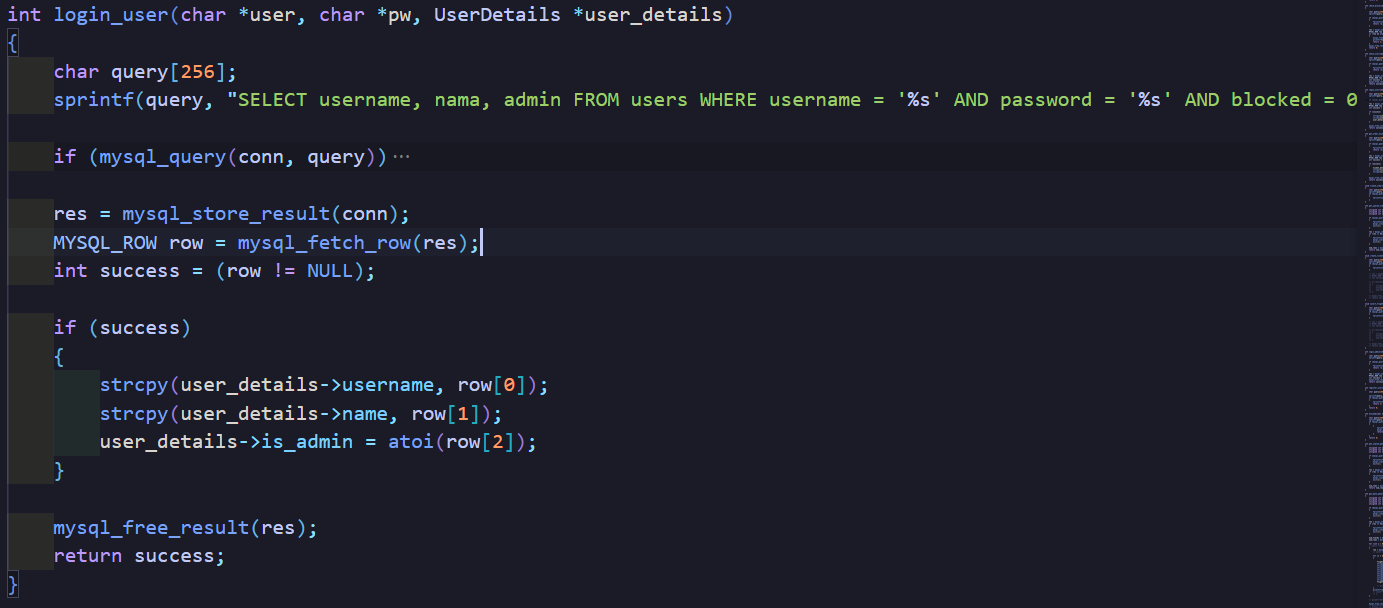
\includegraphics[width=0.5\textwidth]{./img/login_user_mysql.png}
    \caption{fungsi \texttt{\detokenize{login_user()}}}
\end{figure}
\FloatBarrier
fungsi \texttt{\detokenize{login_user()}} membutuhkan 3 argumen, pada argumen yang ke satu dan dua digunakan untuk menginputkan username dan password kemudian untuk argumen ke 3 adalah sebuah struct yang digunakan nantinya untuk menyimpan username nama dan isAdmin.
kemudian terdapat percabangan if didalam if yang pertama digunakan untuk mengecek apakah user ini keblokir atau tidak.
jika ke blokir maka akan menampilkan alert pada GtkLabel kemudian kemudian pada else if dibawahnya mengecek jika hasil == 0  jika iya berarti password yang dimasukanoleh si user salah dan try yang bernilai 3 akan di kurangi 1.
kemudian pada else if dibawahnya digunaka untuk mengecek apakah hasl ==1 jika iya maka windows selanjunya akan di tampilkan.
\begin{figure}[!htbp]
    \centering
    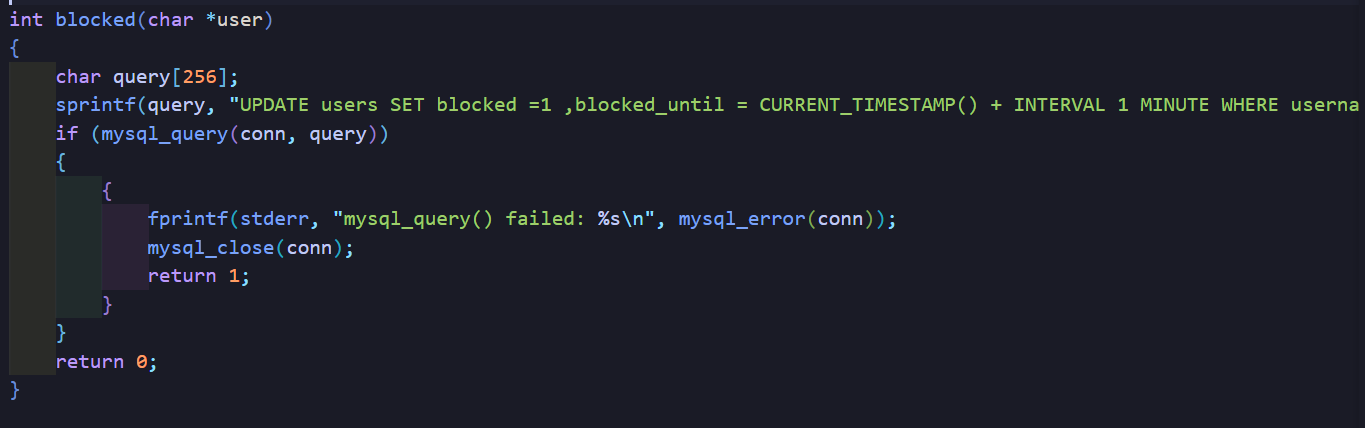
\includegraphics[width=0.5\textwidth]{./img/blocked_mysql.png}
    \caption{fungsi \texttt{\detokenize{blocked()}}}
\end{figure}
\FloatBarrier
fungsi \texttt{\detokenize{blocked()}} digunakan untuk memblokir sementara jika user lebih dari 3x gagal dalam memasukan password. 
\subsection{Login Admin}
Halaman ini adalah halaman untuk login admin 
\begin{figure}[!htbp]
    \centering
    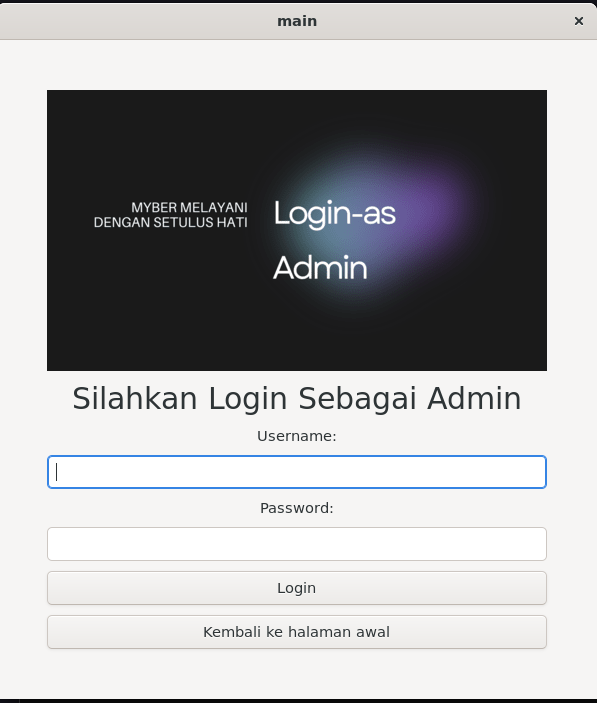
\includegraphics[width=0.5\textwidth]{./img/login_admin/tapilan_login.png}
    \caption{Tampilan Login Admin}
\end{figure}
\FloatBarrier
Pada Halaman login ini digunakan admin untuk login ke halaman dashboard admin. pada halaman ini 
admin diperintahkan untuk memasukkan username dan password untuk login jika username yang di inputkan salah maka akan menampilkan username/ password salah seperti berikut

\begin{figure}[!htbp]
    \centering
    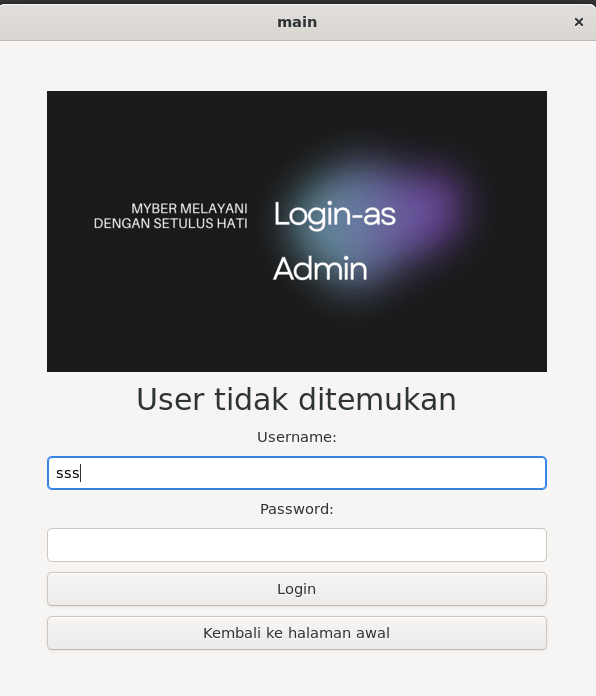
\includegraphics[width=0.5\textwidth]{./img/login_admin/user_not_found.png}
    \caption{Username atau Password salah}
\end{figure}
\begin{figure}[!htbp]
    \centering
    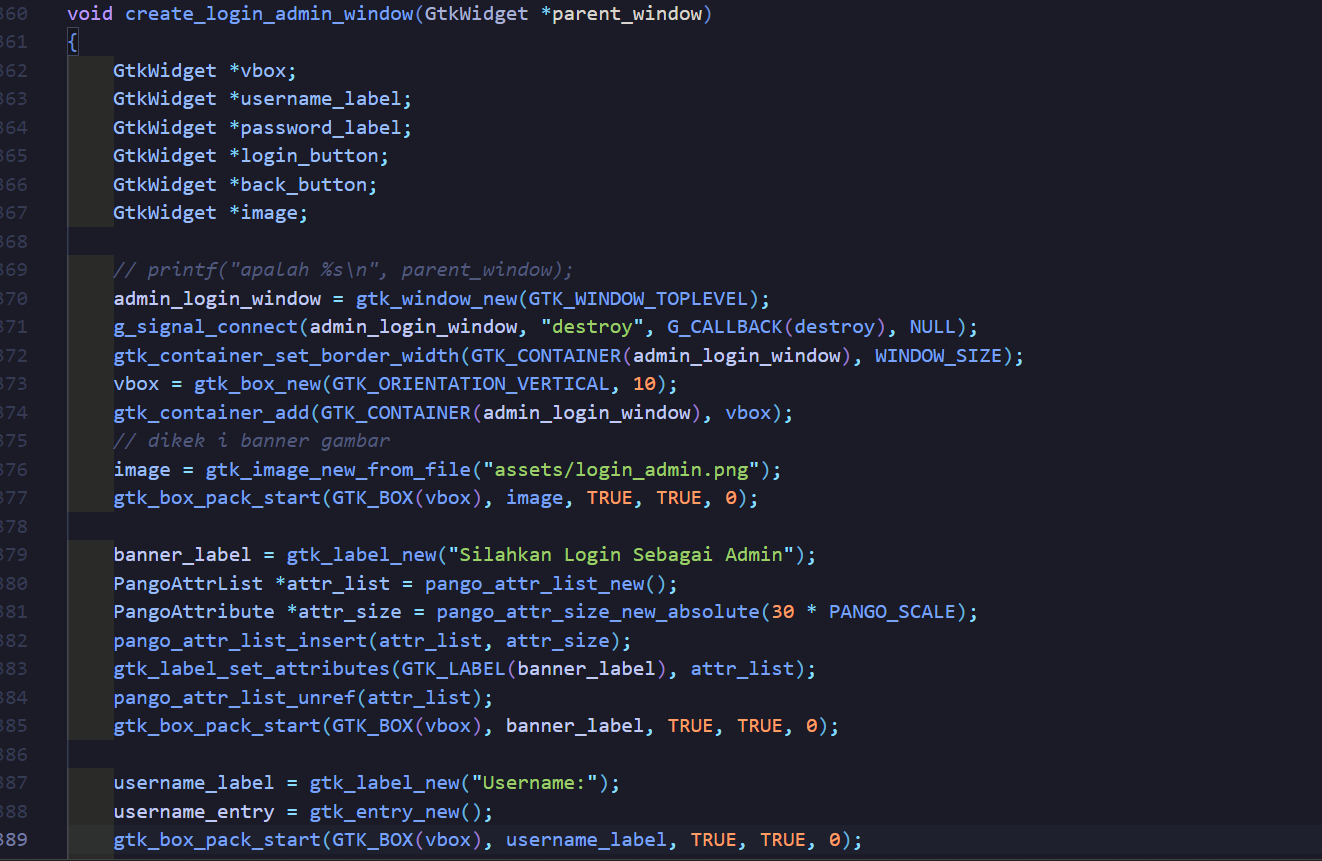
\includegraphics[width=0.5\textwidth]{./img/login_admin/login_window.png}
    \caption{Tampilan Login Admin}
\end{figure}
\FloatBarrier
Pada kode diatas adalah kode untuk membuat window untuk ditampilkan, cara kerjanya sama seperti login user yaitu membuat 
window terlebih dahulu kemudian membuat box vertikal kemudian box vertikal itu dimasukan kedalam window
untuk menampilkan teks pada gtk dapat menggunakan fungsi dari gtk itu sendiri yaitu dengan fungsi \texttt{\detokenize{gtk_label_new()}} kemudian
untuk memberikan ruang teks input pada gtk dapat menggunakan fungsi \texttt{\detokenize{gtk_entry_new()}}, kemudian untuk membuat sebuah button pada gtk dapat 
menggunakan fungsi \texttt{\detokenize{gtk_entry_new()}} dari gtk widget yang sudah dibuat tadi kemudian dimasukan kedalam box vertikal tadi yang sudah dibuat
untuk membuat button ketika ditekan melakukan sebuah tindakan dapat menggunakan sebuah call yang telah disediakan gtk, dalam call back ini akan mengarahkan
kefungsi \texttt{\detokenize{login_process_admin}}
\begin{figure}[!htbp]
    \centering
    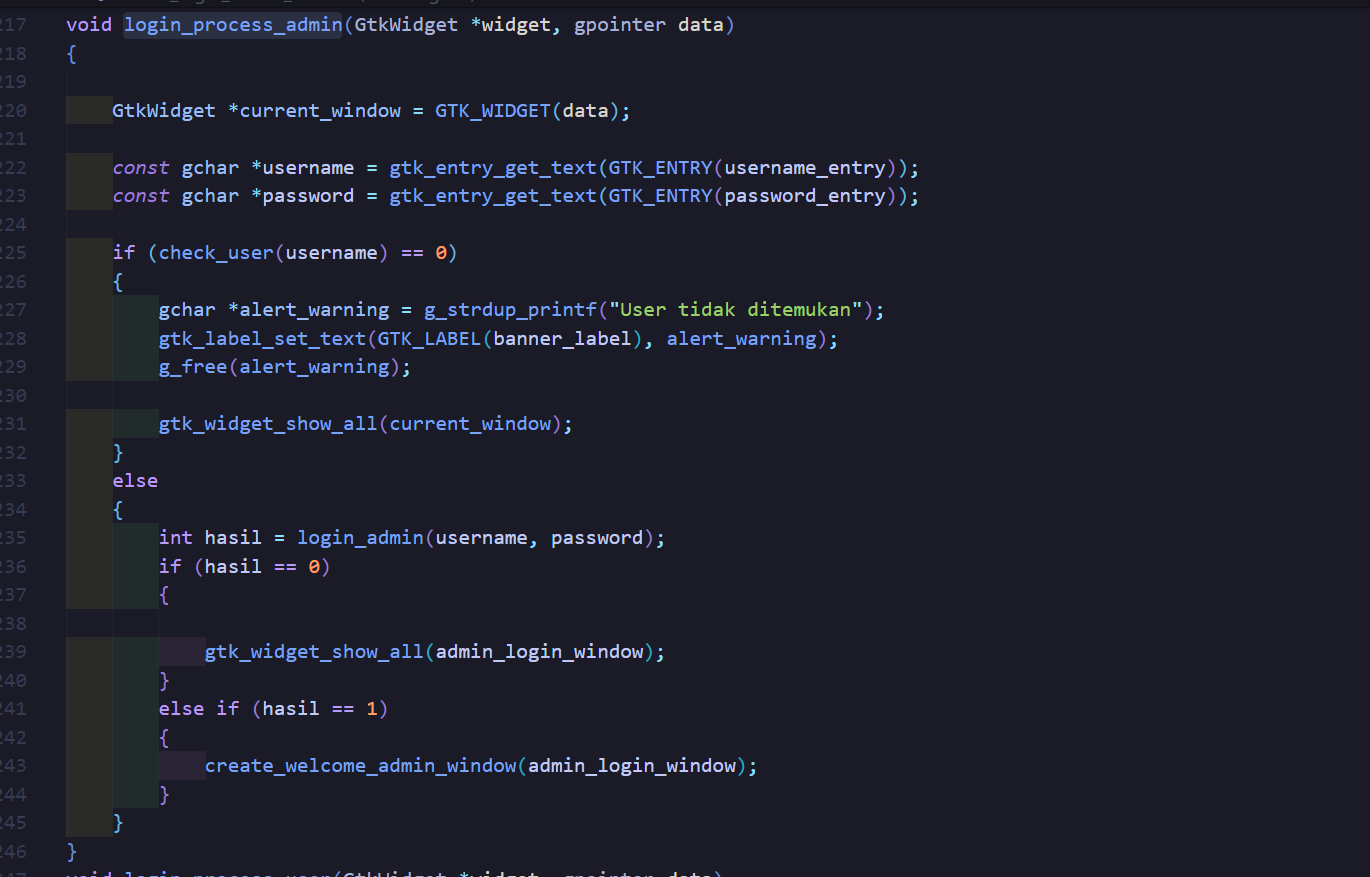
\includegraphics[width=0.5\textwidth]{./img/login_admin/login_proses.png}
    \caption{fungsi \texttt{\detokenize{login_process_admin}}}
\end{figure}
\FloatBarrier
Fungsi ini adalah fungsi yang dipanggil oleh callback button login, dalam fungsi ini digunakan untuk masuk kedalam dashboard admin. didalam fungsi ini terdapat
fungsi check user yang digunakan untuk mengecek username apakah sudah ada didalam database. jika ada maka fungsi \texttt{\detokenize{login_admin()}} akan dieksekusi
\begin{figure}[!htbp]
    \centering
    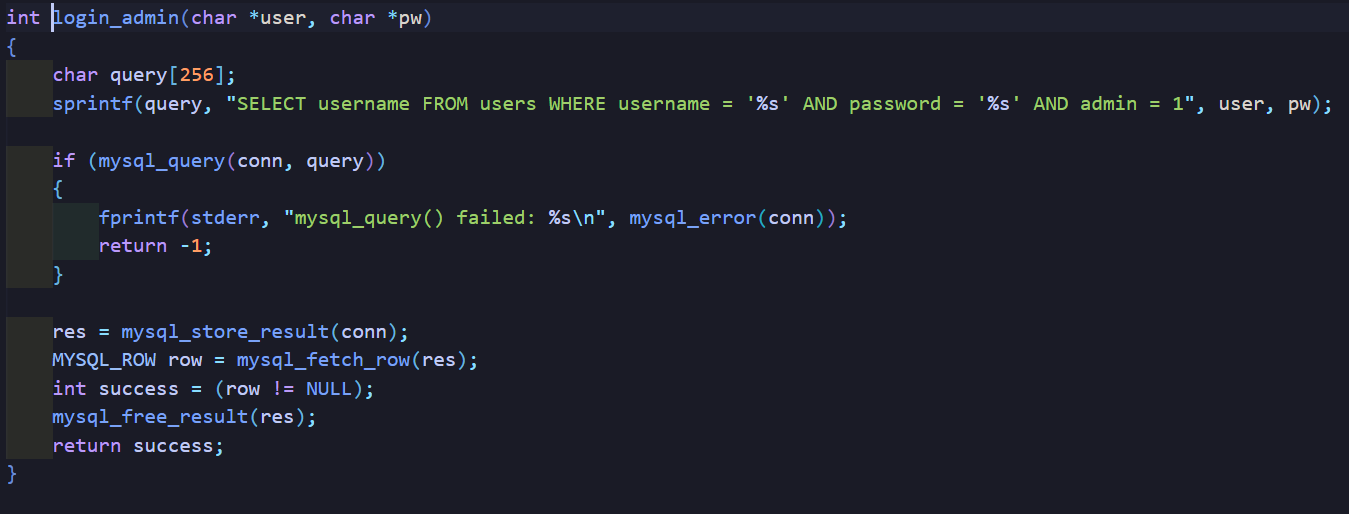
\includegraphics[width=0.5\textwidth]{./img/login_admin/login_mysql.png}
    \caption{fungsi \texttt{\detokenize{login_admin()}}}
\end{figure}
\FloatBarrier
Dalam fungsi \texttt{\detokenize{login_admin()}} ini digunakan untuk mencari username dan password serta isAdmin 1 dari database mysql 
jika pada database ada dan username password dan isAdmin bernilai 1 maka akan diarahkan ke dashboard admin



\subsection{Dashboard Admin}
Ini adalah tampilan dashboard admin
\begin{figure}[!htbp]
    \centering
    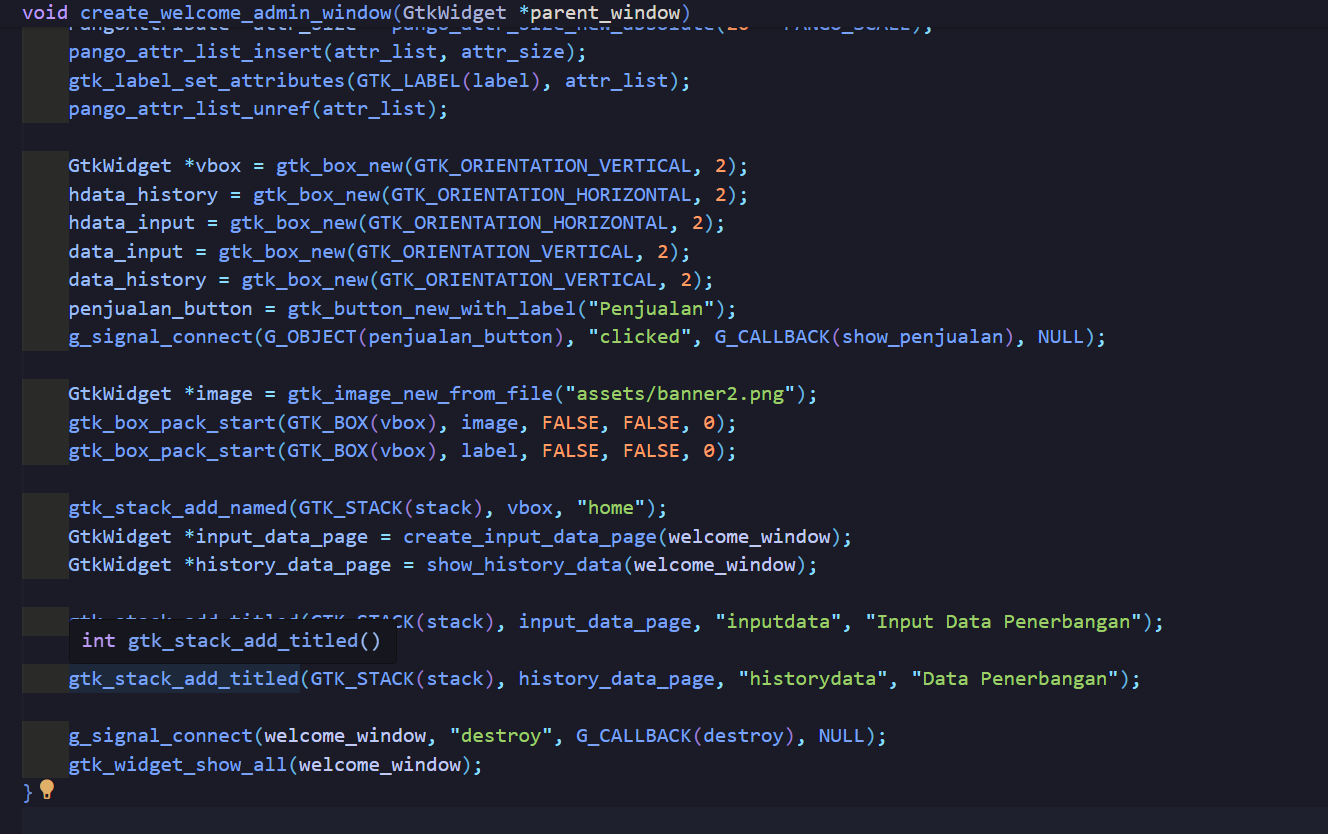
\includegraphics[width=0.5\textwidth]{./img/dashboard admin/kode_dahboard_admin.png}
    \caption{fungsi \texttt{\detokenize{login_admin()}}}
\end{figure}
\section{Kesimpulan}
Keseluruhan alur dari program ini merupakan sebuah manajemen data tiket pesawat oleh dua tipe pengguna.
Dari sisi Admin bertugas sebagai orang yang menginput data penjualan tiket. Sedangkan dari sisi Customer yang akan membeli tiket yang telah diinputkan oleh Admin sebelumnya.
Pada mekanisme Login, Customer bisa melakukan Register dan Login sedangkan Admin hanya bisa melakukan Login karena kredensial dari Admin sendiri sudah dibuatkan dari database. Selain itu, terdapat mekanisme untuk melakukan blocking atau ban
sementara apabila pengguna salah memasukkan passwordnya lebih dari 3 kali, hal ini dilakukan untuk mengantisipasi adanya fraud atau spam. Lalu terdapat error handling yang lain seperti ketika memasukkan User yang belum ada.

\end{document}
